% This is "sig-alternate.tex" V2.1 April 2013
% This file should be compiled with V2.5 of "sig-alternate.cls" May 2012
%
% This example file demonstrates the use of the 'sig-alternate.cls'
% V2.5 LaTeX2e document class file. It is for those submitting
% articles to ACM Conference Proceedings WHO DO NOT WISH TO
% STRICTLY ADHERE TO THE SIGS (PUBS-BOARD-ENDORSED) STYLE.
% The 'sig-alternate.cls' file will produce a similar-looking,
% albeit, 'tighter' paper resulting in, invariably, fewer pages.
%
% ----------------------------------------------------------------------------------------------------------------
% This .tex file (and associated .cls V2.5) produces:
%       1) The Permission Statement
%       2) The Conference (location) Info information
%       3) The Copyright Line with ACM data
%       4) NO page numbers
%
% as against the acm_proc_article-sp.cls file which
% DOES NOT produce 1) thru' 3) above.
%
% Using 'sig-alternate.cls' you have control, however, from within
% the source .tex file, over both the CopyrightYear
% (defaulted to 200X) and the ACM Copyright Data
% (defaulted to X-XXXXX-XX-X/XX/XX).
% e.g.
% \CopyrightYear{2007} will cause 2007 to appear in the copyright line.
% \crdata{0-12345-67-8/90/12} will cause 0-12345-67-8/90/12 to appear in the copyright line.
%
% ---------------------------------------------------------------------------------------------------------------
% This .tex source is an example which *does* use
% the .bib file (from which the .bbl file % is produced).
% REMEMBER HOWEVER: After having produced the .bbl file,
% and prior to final submission, you *NEED* to 'insert'
% your .bbl file into your source .tex file so as to provide
% ONE 'self-contained' source file.
%
% ================= IF YOU HAVE QUESTIONS =======================
% Questions regarding the SIGS styles, SIGS policies and
% procedures, Conferences etc. should be sent to
% Adrienne Griscti (griscti@acm.org)
%
% Technical questions _only_ to
% Gerald Murray (murray@hq.acm.org)
% ===============================================================

\documentclass{sig-alternate}

\usepackage{mathtools}
\usepackage[urlbordercolor={1 1 1},citebordercolor={1 1 1},linkbordercolor={1 1 1}]{hyperref}
\usepackage{enumitem}
\usepackage{tikz}
\usetikzlibrary{decorations.text}
\usepackage{tkz-berge}
\usepackage{amsmath}

% https://tex.stackexchange.com/questions/42271/floor-and-ceiling-functions
\DeclarePairedDelimiter{\ceil}{\lceil}{\rceil}
\DeclarePairedDelimiter{\floor}{\lfloor}{\rfloor}

\newcommand*\concat{\mathbin{\|}}

\begin{document}

% Copyright
\setcopyright{acmcopyright}
%\setcopyright{acmlicensed}
%\setcopyright{rightsretained}
%\setcopyright{usgov}
%\setcopyright{usgovmixed}
%\setcopyright{cagov}
%\setcopyright{cagovmixed}

% DOI
\doi{10.475/123_4}

% ISBN
\isbn{123-4567-24-567/08/06}

%Conference
\conferenceinfo{ACM CCS '15}{October 12-16, 2015, Denver, Colorado, USA}

\acmPrice{\$15.00}

% --- Author Metadata here ---
%\conferenceinfo{WOODSTOCK}{'97 El Paso, Texas USA}
\CopyrightYear{2015} % Allows default copyright year (20XX) to be over-ridden - IF NEED BE.
%\crdata{0-12345-67-8/90/01}  % Allows default copyright data (0-89791-88-6/97/05) to be over-ridden - IF NEED BE.
% --- End of Author Metadata ---

\title{The Onion Name System}
\subtitle{Tor-powered Distributed DNS for Tor Hidden Services}

\numberofauthors{3}
\author{
	[anonymous submission]
%% 1st. author
%\alignauthor
%Jesse Victors \\
%       \affaddr{7449 S. Babcock Blvd.}\\
%       \affaddr{Wasilla, AK 99623}\\
%       \email{jvictors@jessevictors.com}
%% 2nd. author
%\alignauthor
%Ming Li\\
%       \affaddr{Utah State University}\\
%       \affaddr{Logan, UT 84321}\\
%       \email{ming.li@usu.edu}
%% 3rd. author
%\alignauthor
%Xinwen Fu\\
%       \affaddr{University of Massachusetts Lowell}\\
%       \affaddr{Lowell, MA 01854 }\\
%       \email{xinwenfu@cs.uml.edu}
}

\maketitle

\begin{abstract}

Tor hidden services are anonymous servers of unknown location and ownership who can be accessed through any Tor-enabled web browser. They have gained popularity over the years, but still suffer from major usability challenges due to their cryptographically-generated non-memorable addresses.

In response to this difficulty, in this work we introduce the Onion Name System (OnioNS), a privacy-enhanced distributed DNS that allows users to reference a hidden service by a meaningful globally-unique verifiable domain name chosen by the hidden service operator. We introduce a new distributed self-healing public ledger and construct OnioNS as an optional backwards-compatible plugin for Tor on top of existing hidden service infrastructure. We simplify our design and threat model by embedding OnioNS within the Tor network and provide mechanisms for authenticated denial-of-existence with minimal networking costs. Our reference implementation demonstrates that OnioNS successfully addresses the major usability issue that has been with Tor hidden services since their introduction in 2002.

\end{abstract}

%% http://dl.acm.org/ccs.cfm
%% http://www.acm.org/about/class/
%% https://academia.stackexchange.com/questions/15252/is-the-new-acm-2012-taxonomy-usable-in-use
%\begin{CCSXML}
%<ccs2012>
%<concept>
%<concept_id>10002951.10003152.10003161.10003164</concept_id>
%<concept_desc>Information systems~Block / page strategies</concept_desc>
%<concept_significance>500</concept_significance>
%</concept>
%<concept>
%<concept_id>10003033.10003099.10003037</concept_id>
%<concept_desc>Networks~Naming and addressing</concept_desc>
%<concept_significance>500</concept_significance>
%</concept>
%<concept>
%<concept_id>10002978.10003006.10003013</concept_id>
%<concept_desc>Security and privacy~Distributed systems security</concept_desc>
%<concept_significance>300</concept_significance>
%</concept>
%<concept>
%<concept_id>10002978.10002979</concept_id>
%<concept_desc>Security and privacy~Cryptography</concept_desc>
%<concept_significance>100</concept_significance>
%</concept>
%<concept>
%<concept_id>10002978.10003014.10003015</concept_id>
%<concept_desc>Security and privacy~Security protocols</concept_desc>
%<concept_significance>100</concept_significance>
%</concept>
%</ccs2012>
%\end{CCSXML}
%
%\ccsdesc[500]{Information systems~Block / page strategies}
%\ccsdesc[500]{Networks~Naming and addressing}
%\ccsdesc[300]{Security and privacy~Distributed systems security}
%\ccsdesc[100]{Security and privacy~Cryptography}
%\ccsdesc[100]{Security and privacy~Security protocols}

%{Security and privacy}
%	Cryptography
%	Systems security
%		Distributed systems security
%	 Network security
%	 	Security protocols
%{Information systems}
%	{Information storage systems}
%		Record storage systems
%			Block / page strategies
%{Networks}
%	Network services
%		Naming and addressing

%\printccsdesc

\category{C.2.0}{Computer Communications Networks}{Security and protection}
\category{C.2.4}{Computer Communications Networks}{Distributed Systems}[Client/server, Distributed databases]
\category{E.1}{Data Structures}{Distributed data structures}[Records]

\keywords{Tor, onion, hidden service, anonymity, privacy, network security, petname}

\section{Introduction}

As the prevalence of the Internet and other communication has grown, so too has the development and usage of privacy-enhancing systems. These are protocols that provide privacy by obfuscating the link between a user's identity or location and their communications. Following a general distrust of unsecured Internet communications and in light of the 2013-current revelations by Edward Snowden of international Internet mass-surveillance, users have increasingly turned to these tools for their own protection.

Tor\cite{dingledine2004tor} is a third-generation onion routing system and is the most popular low-latency anonymous communication network in use today. In Tor, users construct a layered encrypted communications circuit over three onion routers in order to mask their identity and location. As messages travel through the circuit, each onion router in turn decrypts their encryption layer, exposing their respective routing information. This provides end-to-end communication confidentiality of the sender.

Tor users interact with the Internet and other systems over Tor via the Tor Browser, a security-enhanced fork of Firefox ESR. This achieves a level of usability but also security: Tor achieves most of its application-level sanitization via privacy filters in the Tor Browser; unlike its predecessors, Tor performs little sanitization itself. Tor's threat model assumes that the capabilities of adversaries are limited to traffic analysis attacks on a restricted scale; they may observe or manipulate portions of Tor traffic, that they may run onion routers themselves, and that they may compromise a fraction of other existing routers. Tor's design centers around usability and defense against these types of attacks.

\subsection{Motivation}

Tor also supports \emph{hidden services} -- anonymous servers that intentionally mask their IP address through Tor circuits. They utilize the .onion pseudo-TLD, preventing hidden services from being accessed outside the context of Tor. Hidden services are only known by their public RSA key and typically referenced by their address, 16 base32-encoded characters derived from the SHA-1 hash of the server's key. This builds a publicly-confirmable one-to-one relationship between the public key and its address and allows hidden services to be accessed via the Tor Browser by their address within a distributed environment.

\begin{figure}[htbp]
	\centering
	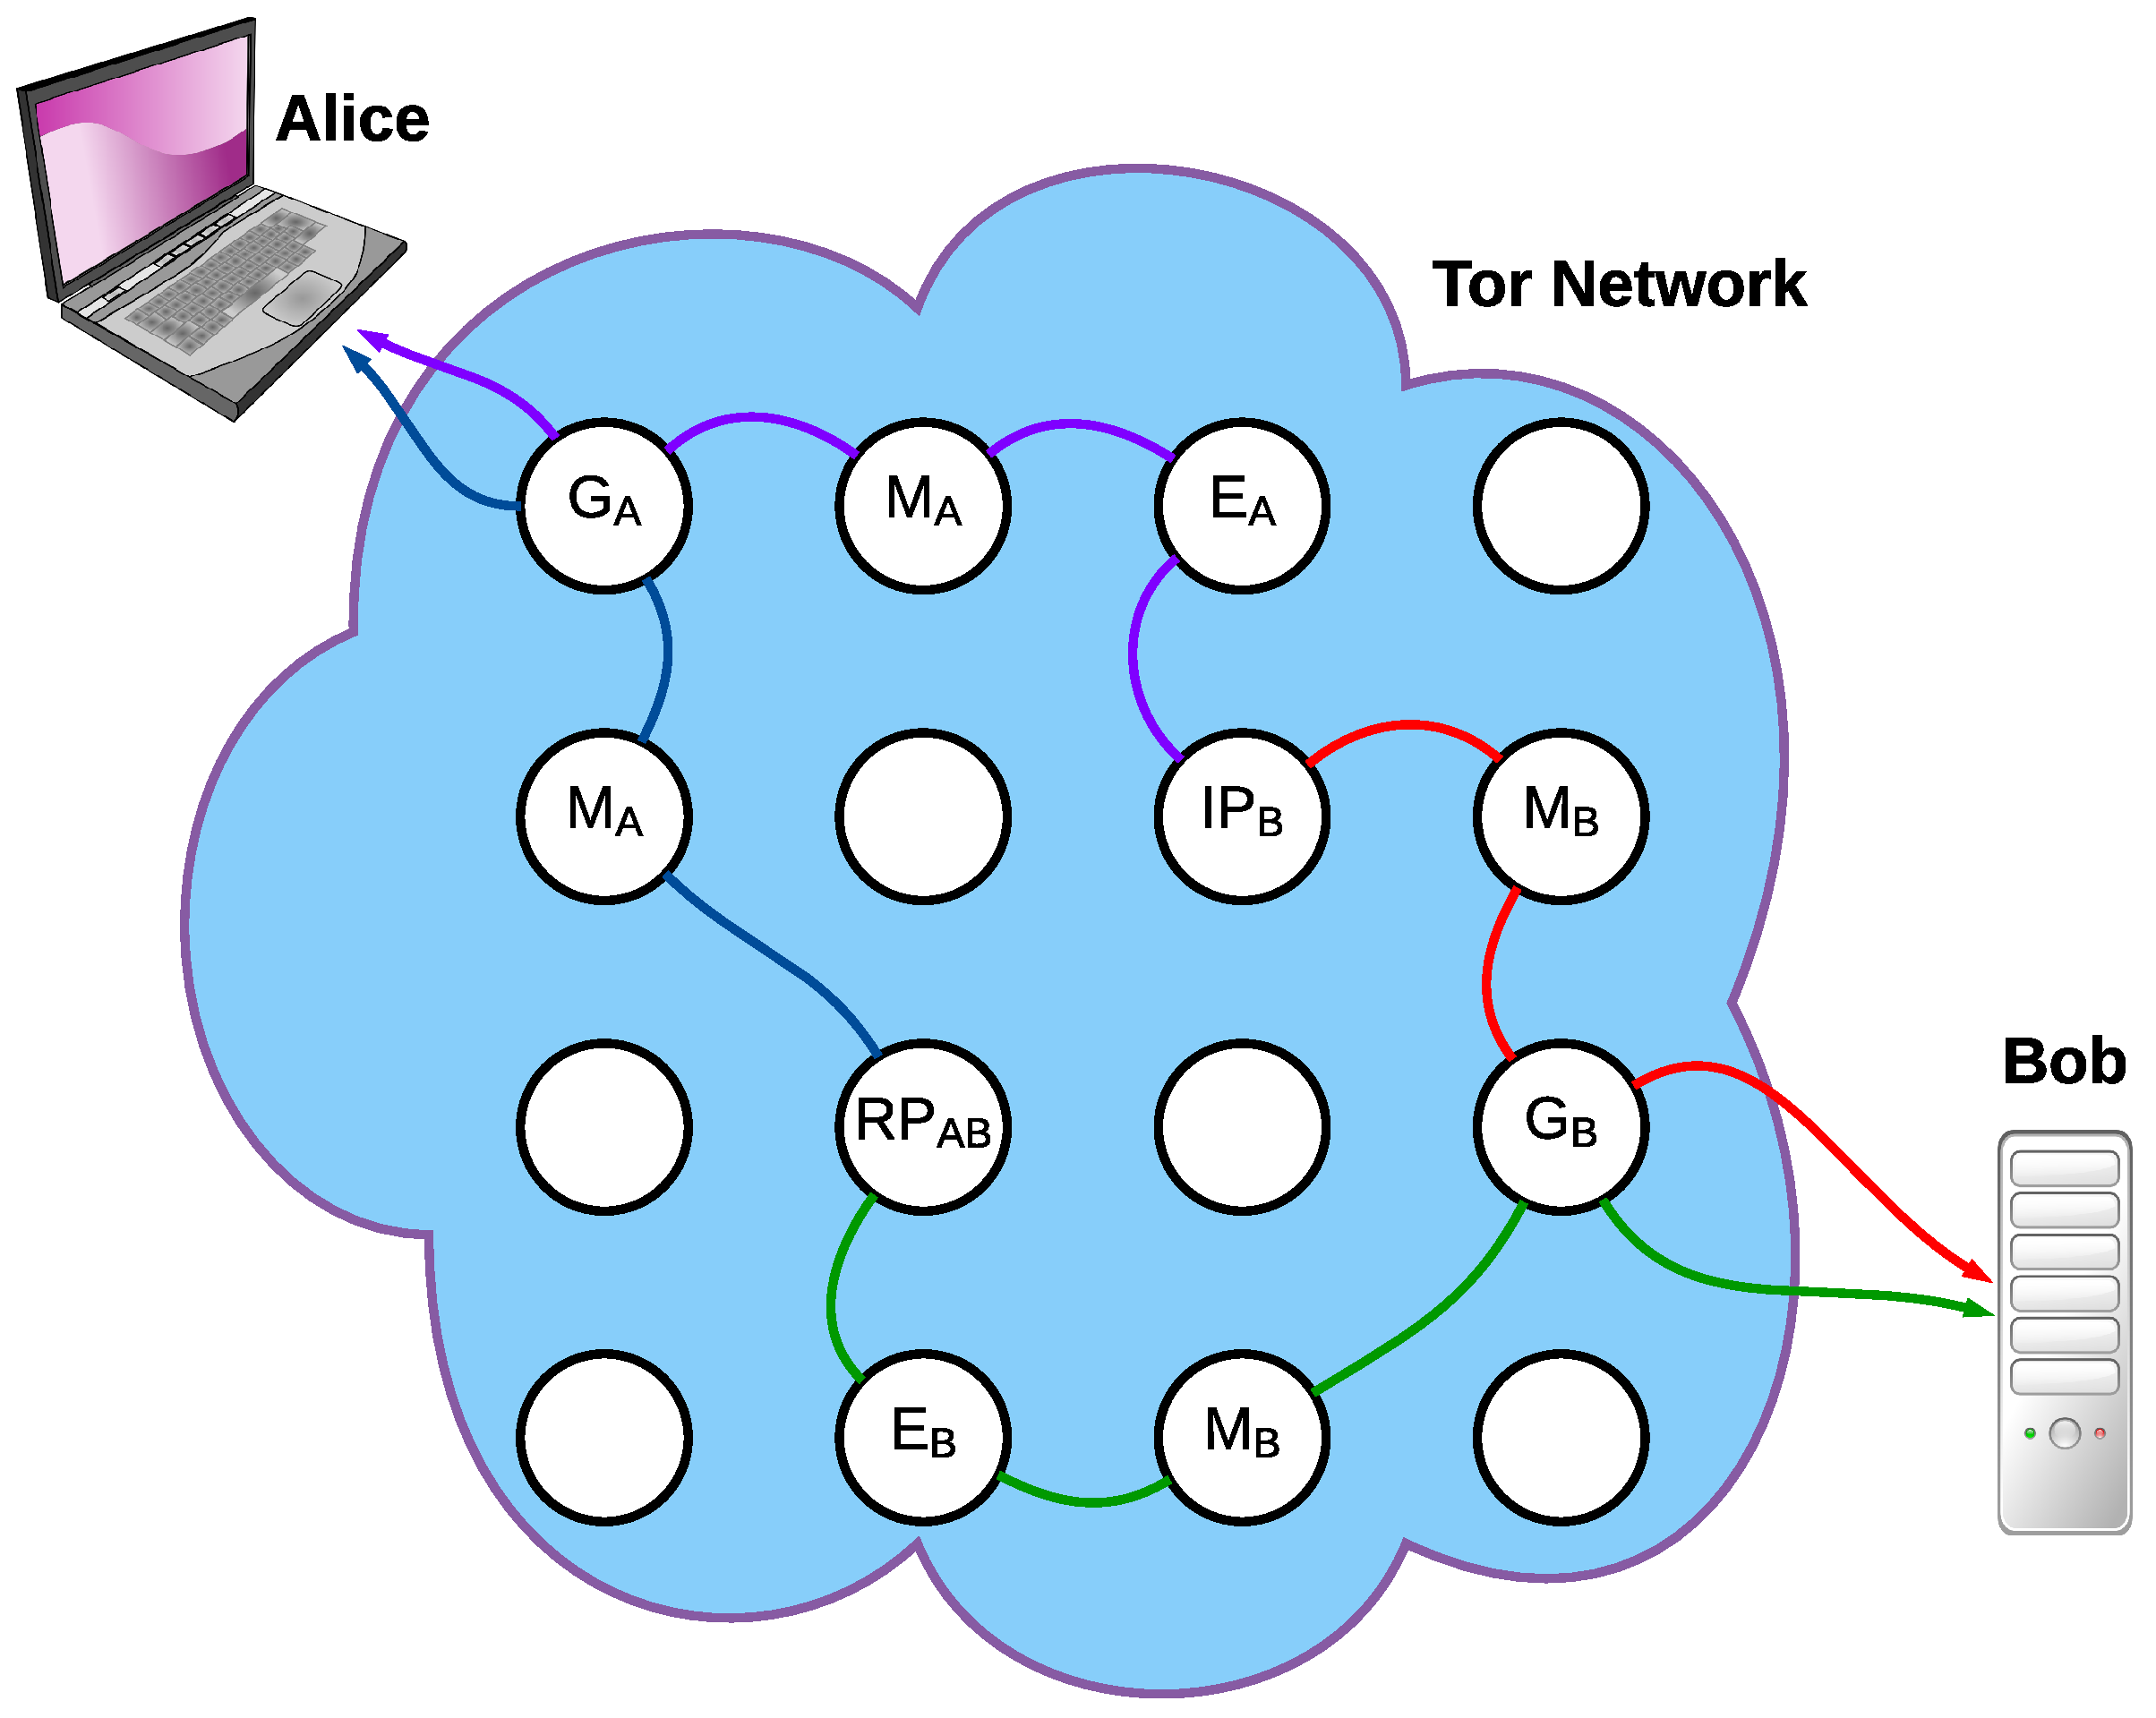
\includegraphics[width=0.9\linewidth]{../images/LucidCharts/Hidden_Services.pdf}
	\caption{A Tor client, Alice, and a hidden service, Bob, first mate two Tor circuits (purple and red) at one of Bob's long-term \emph{introduction points} (IP). They then renegotiate and communicate over another pair of Tor circuits (blue and green) at an ephemeral \emph{rendezvous point} (RP). This achieves communication with bi-directional anonymity.\cite{overlier2006locating}}
\end{figure}

Tor hidden service addresses are distributed and globally collision-free, but there is a strong discontinuity between the address and the service's purpose. For example, a visitor cannot determine that \url{3g2upl4pq6kufc4m.onion} is the DuckDuckGo search engine without visiting the hidden service. Generally speaking, it is currently impossible to categorize or fully label hidden services in advance. Over time, third-party directories -- both on the Clearnet and Darknet -- have appeared in attempt to counteract this issue, but these directories must be constantly maintained and the approach is neither convenient nor does it scale well. Given the approximetly 25,000 hidden services on the Tor network,  (Figure \ref{fig:OnionCount}) this suggests the strong need for a more complete solution to solve the usability issue.

\begin{figure}[htbp]
	\centering
	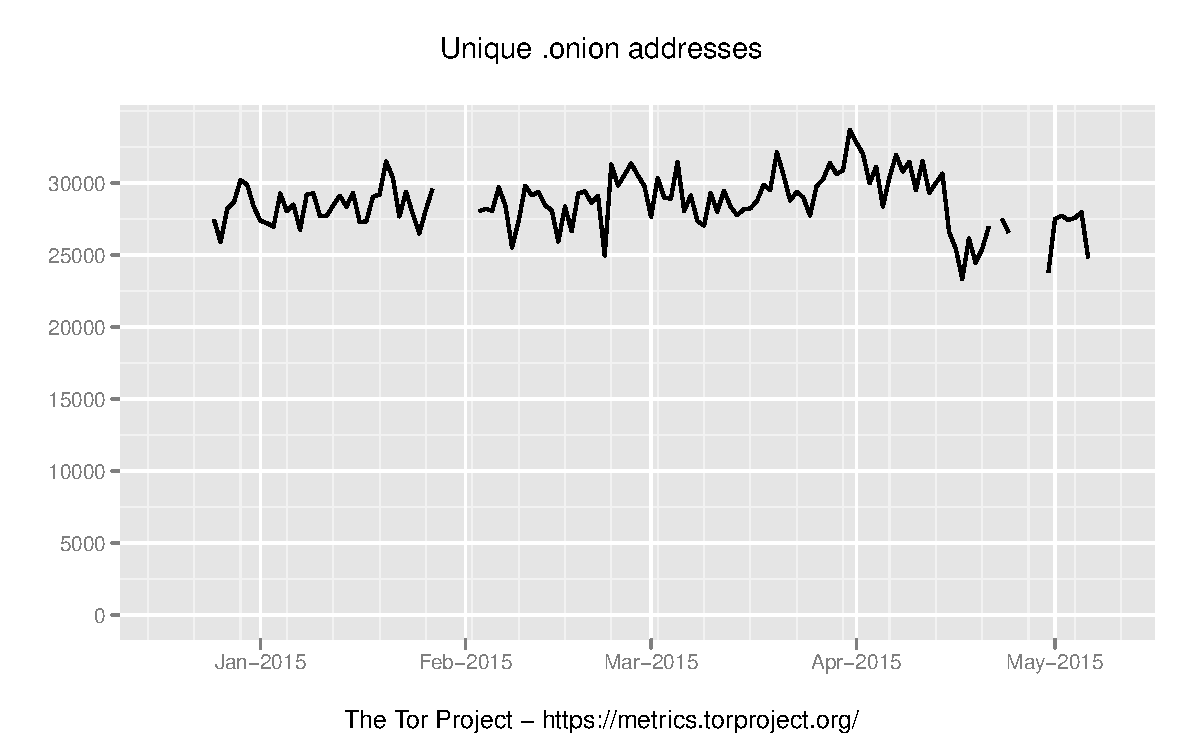
\includegraphics[width=0.95\linewidth]{../images/Tor/onion_2014-10_2015-05.pdf}
	\caption{The number of unique .onion addresses seen in the Tor network between December 2014 and May 2015.\cite{kadianakis2015extrapolating}\cite{TorMetrics}}
	\label{fig:OnionCount}
\end{figure}

\subsection{Contributions}

In this paper, we present the design, analysis and implementation of the Onion Name System, (OnioNS) a distributed, secure, and usable domain name system for Tor hidden services. Any hidden service can anonymously register an association between a meaningful human-readable domain name and its .onion address and clients can query against OnioNS in a privacy-preserving and verifiable manner. OnioNS is powered by a random subset of nodes within the existing infrastructure of Tor, significantly limiting the additional attack surface. We devise a distributed DNS database using a blockchain-based data structure that is tamper-proof, self-healing, resistant to node compromise, and provides authenticated denial-of-existence. We design OnioNS as a backwards-compatible plugin to the Tor software. Our prototype implementation demonstrates the high usability and performance of OnioNS. To the best of our knowledge, this is the first alternative DNS for Tor hidden services which is distributed, secure, and usable at the same time.

\textbf{Paper Organization:} This paper is divided into four main sections. In section \ref{sec:problemStatement} we define our design objectives and explain why existing works do not meet our goals. We also define our threat model, which closely matches Tor's model with one additional assumption. In section \ref{sec:Solution}, we describe the system overview and define several key protocols. In section \ref{sec:Analysis} we analyse the security of our assumptions and examine other attack vectors. Last, in section \ref{sec:Analysis} we evaluate our implementation prototype and show that it can access a hidden service under a meaningful domain name.

\section{Problem Statement}
\label{sec:problemStatement}

To integrate with Tor, we must provide a secure system, preserve user privacy, and avoid compromising other areas of the Tor network. Additionally, we seek to achieve all three properties of Zooko's Triangle (section \ref{sec:ZookosTriangle}) and to providing a mechanism for authenticated denial-of-existence (section \ref{sec:authDenialIntro}).

\subsection{Design Objectives}

Here we enumerate a list of requirements that must be met by any DNS applicable to Tor hidden services. In Section \ref{sec:RelatedWorks} we analyse existing works and show how these systems do not meet these requirements and in Section \ref{sec:Solution} we demonstrate how we overcome them with OnioNS.

1. \textbf{The system must support anonymous registrations.} The system should not require any personally-identifiable or location information from the registrant. Tor hidden services publicize no more information than a public key and Introduction Points.

2. \textbf{The system must support privacy-enhanced queries.} Clients should be anonymous, indistinguishable, and unable to be tracked by name servers.

3. \textbf{Registrations must be authenticable.} Clients must be able to verify that the domain-address pairing that they receive from name servers is authentic relative to the authenticity of the hidden service.

4. \textbf{Domain names must be globally unique.} Any domain name of global scope must point to at most one server. For naming systems that generate names via cryptographic hashes, the key-space must be of sufficient length to resist cryptanalytic attack.

5. \textbf{The system must be distributed.} Systems with root authorities have distinct disadvantages compared to distributed networks: specifically, central authorities have absolute control over the system and root security breaches could easily compromise the integrity of the entire system. Root authorities may also be able to compromise the privacy of both users and hidden services or may not allow anonymous registrations.

6. \textbf{The system must be relatively easy to use.} It should be assumed that users are not security experts or have technical backgrounds. The system must resolve protocols with minimal input from the user and hide non-essential details.

7. \textbf{The system must be backwards compatible.} Naming systems for Tor must preserve the original Tor hidden service protocol, making the DNS optional but not required.

8. \textbf{The system should be lightweight.} In most realistic environments clients have neither the bandwidth nor storage capacity to hold the system's entire database, nor the capability of meeting significant computation burdens.

\subsection{Challenges}

\subsubsection{Zooko's Triangle}
\label{sec:ZookosTriangle}

In 2001, Zooko Wilcox-O'Hearn described three desirable properties for any persistent naming system: distributed design, assignment of human-meaningful names, and globally unique names. In a statement now known as Zooko's Triangle,\cite{ferdous2009security}\cite{stiegler2005petname} he claimed any naming system could only achieve two of these properties. This is illustrated in Figure \ref{fig:ZookosTriangle}.

\begin{figure}[htbp]
	\centering
	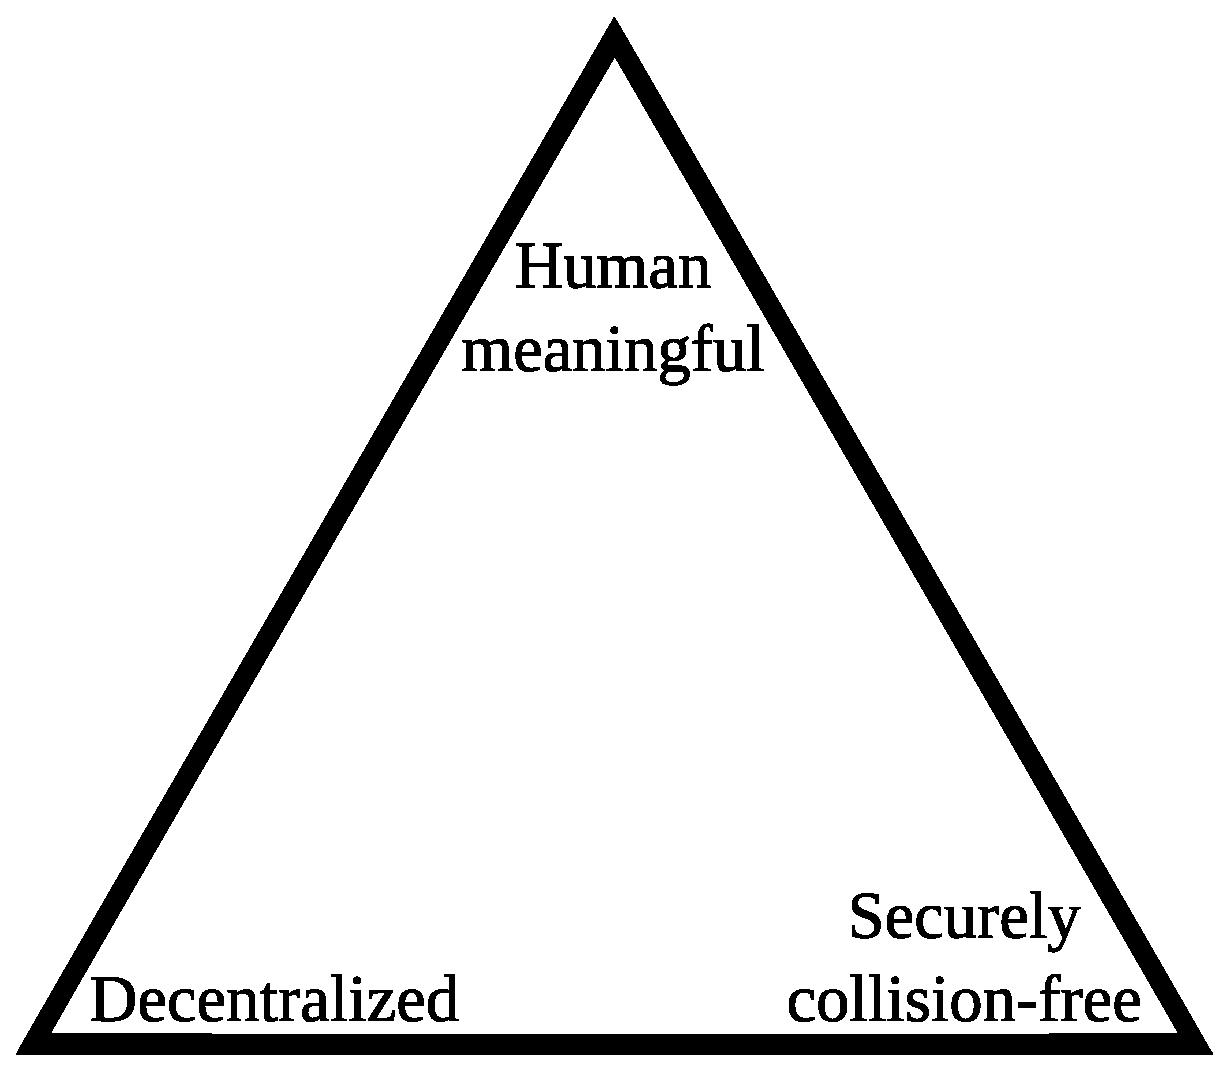
\includegraphics[width=0.3\textwidth]{../images/Zooko.eps}
	\caption{Zooko's Triangle.}
	\label{fig:ZookosTriangle}
\end{figure}

Some examples of naming systems that achieve only two of these properties include:

\begin{itemize}[noitemsep]
	\item \textbf{Securely unique and human-meaningful} \\ --- Internet domain names and GNS.
	\item \textbf{Decentralized and human-meaningful} \\ --- Human names and nicknames.
	\item \textbf{Securely unique and decentralized} \\ --- Tor hidden service .onion addresses.
\end{itemize}

% Petnames, such as Namecoin and OnioNS, are systems that achieve all three properties of Zooko's Triangle.

\subsubsection{Authenticated Denial-of-Existence}
\label{sec:authDenialIntro}

If a naming system provides authentication, clients should be able to verify the authenticity of existing domain names and authenticate a denial-of-existence claim by their name server. On the Internet, the former is addressed by SSL certificates and a chain of trust to root Certificate Authorities, while the latter remains a possible attack vector. DNSSEC includes an extension for Hashed Authenticated Denial of Existence (NSEC3) which provides signed non-existence claims on a per-domain basis. However, DNSSEC has not seen widespread use, storing per-domain denial-of-existence records introduces significant storage requirements, and to our knowledge no alternative DNS provides mechanisms for authenticated denial-of-existence. Closing this attack vector is not easy; the na\"{i}ve solution of generating proof individually or en-masse for every non-existent domain is infeasible since the number of possible domain names is likely too large to practically enumerate.

\section{Related Works}
\label{sec:RelatedWorks}

Vanity key generators (e.g. Shallot\cite{KatmagicShallot}) attempt to find by brute-force an RSA key that generates a partially-desirable hash. Vanity key generators are commonly used by hidden service operators to improve the recognition of their hidden service, particularly for higher-profile services.\cite{syversongenuine} For example, a hidden service operator may wish to start his service's address with a meaningful noun so that others may more easily recognize it. However, these generators are only partially successful at enhancing readability because the size of the domain key-space is too large to be fully brute-forced in any reasonable length of time. If the address key-space was reduced to allow a full brute-force, the system would fail to be guaranteed collision-free. Nicolussi suggested changing the address encoding to a delimited series of words, using a dictionary known in advance by all parties.\cite{nicolussi2011human} Like vanity key generators, Nicolussi's encoding partially improves the recognition and readability of an address but does nothing to counter the large key-space nor alleviate the logistic problems of manually entering in the address into the Tor Browser. These attempts are purely cosmetic and do not qualify as a full solution.

The Internet DNS is another one candidate and is already well established as a fundamental abstraction layer for Internet routing. However, despite its widespread use and extreme popularity, the Internet DNS suffers from several significant shortcomings and fundamental security issues that make it inappropriate for use by Tor hidden services. With the exception of extensions such as DNSSEC, the Internet DNS by default does not use any cryptographic primitives. DNSSEC is primarily designed to prevent forgeries and DNS cache poisoning from intermediary name servers and it does not provide any degree of query privacy.\cite{wachs2014censorship} Additional extensions and protocols such as DNSCurve\cite{bernstein2009dnscurve} have been proposed, but DNSSEC and DNSCurve are optional and have not yet seen widespread full deployment across the Internet. The lack of default security in Internet DNS and the financial expenses involved with registering a new TLD casts significant doubt on the feasibility of using it for Tor hidden services. Cachin and Samar\cite{cachin2004secure} extended the Internet DNS and decreased the attack potential for authoritative name servers via threshold cryptography, but the lack of privacy in the Internet DNS and the logistical difficulty in globally implementing their work prevents us from using their system for hidden services.

The GNU Name System\cite{wachs2014censorship} (GNS) is another zone-based alternative DNS. GNS describes a hierarchical zones of names with each user managing their own zone and distributing zone access peer-to-peer within social circles. While GNS' design guarantees the uniqueness of names within each zone and users are capable of selecting meaningful nicknames for themselves, GNU does not guarantee that names are \emph{globally} unique. Furthermore, the selection of a trustworthy zone to use would be a significant challenge for using GNS for Tor hidden services and such a selection no longer makes the system distributed. Awerbuch and Scheideler,\cite{awerbuch2004group} constructed a distributed peer-to-peer naming system, but like GNS, made no guarantee that domain names would be globally unique.

% \cite{jacobs2014providing} was

Namecoin\cite{NamecoinHome} is an early fork of Bitcoin\cite{nakamoto2008bitcoin} and is noteworthy for achieving all three properties of Zooko's Triangle. Namecoin holds information transactions in a distributed ledger known as a blockchain. Storing textual information such as a domain registration consumes some Namecoins, a unit of currency. While Namecoin is often advertised as capable of assigning names to Tor hidden services, it has several practical issues that make it generally infeasible to be used for that purpose. First, to authenticate registrations, clients must be able to prove the relationship between a Namecoin owner's secp256k1 ECDSA key and the target hidden service's RSA key: constructing this relationship is non-trivial. Second, Namecoin generally requires users to pre-fetch the blockchain which introduces significant logistical issues due to high bandwidth, storage, and CPU load. Third, although Namecoin supports anonymous ownership of information, it is non-trivial to anonymously purchase Namecoins, thus preventing domain registration from being truly anonymous. These issues prevent Namecoin from being a practical alternative DNS for Tor hidden service. However, our work shares some design principles with Namecoin.

\section{Assumptions and Threat Model}
\label{sec:threatModel}

We assume that Tor provides privacy and anonymity; if Alice constructs a three-hop Tor circuit to Bob with modern Tor cryptographic protocols and sends a message $ m $ to Bob, we assume that Bob can learn no more about Alice than the contents of $ m $. This implies that if $ m $ does not contain identifiable information, Alice is anonymous from Bob's perspective, regardless of if $ m $ is exposed to an attacker, Eve. Identifiable information in $ m $ is outside of Tor's scope, but we do not introduce any protocols that cause this scenario.

We assume secure cryptographic primitives; namely that Eve cannot break standard cryptographic primitives such as AES, SHA-2, RSA, Curve25519, Ed25519, and the scrypt key derivation function. We assume that Eve maintains no backdoors or knows secret software breaks in the Botan or the OpenSSL implementations of these primitives.

% deterministic in there for a reason

We assume that not all Tor routers are honest; that Eve controls some percentage of Tor routers such that Eve's routers may actively collude. Routers may also be semi-honest; wiretapped but not capable of violating protocols. However, the percentage of dishonest and semi-honest routers is small enough to avoid violating our first assumption. We assume a fixed percentage of dishonest and semi-honest routers; namely that the percentage of routers under an Eve's control does not increase in response to the inclusion of OnionNS into Tor infrastructure. This assumption simplifies our threat model analysis but we consider it realistic because while Tor traffic is purposely secret as it travels through the network, we consider OnioNS information public so we don't consider the inclusion of OnioNS a motivating factor to Eve.

If $ C $ is a Tor network status consensus, (section \ref{sec:SolutionOverview}) $ Q $ is an $ M $-sized set randomly but deterministically selected from the Fast and Stable routers listed in $ C $, and $ Q $ is under the influence of one or more adversaries, we assume that the largest subset of agreeing routers in $ Q $ are at least semi-honest.

\section{Solution}
\label{sec:Solution}

\subsection{Overview}
\label{sec:SolutionOverview}

\begin{figure}[htbp]
	\centering
	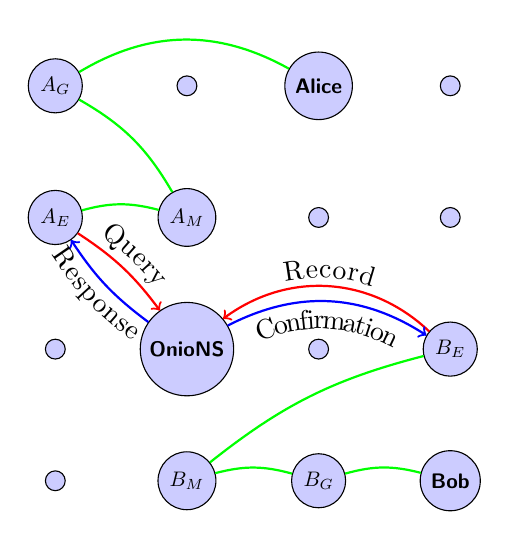
\begin{tikzpicture}[scale=0.76, ->, node distance=2.2cm, main node/.style={circle, fill=blue!20, draw, font=\sffamily\bfseries, transform shape}]

			\node[main node] (1) {$ A_{G} $};
			\node[main node] (2) [right of=1] {};
			\node[main node] (3) [right of=2] {Alice};
			\node[main node] (4) [right of=3] {};

			\node[main node] (5) [below of=1] {$ A_{E} $};
			\node[main node] (6) [right of=5] {$ A_{M} $};
			\node[main node] (7) [right of=6] {};
			\node[main node] (8) [right of=7] {};

			\node[main node] (9) [below of=5] {};
			\node[main node] (10) [right of=9] {OnioNS};
			\node[main node] (11) [right of=10] {};
			\node[main node] (12) [right of=11] {$ B_{E} $};

			\node[main node] (13) [below of=9] {};
			\node[main node] (14) [right of=13] {$ B_{M} $};
			\node[main node] (15) [right of=14] {$ B_{G} $};
			\node[main node] (16) [right of=15] {Bob};

			% Alice-OnioNS conversation
			\tikzstyle{EdgeStyle}=[bend right, -, green]
			\Edge[](3)(1)
			\tikzstyle{EdgeStyle}=[bend left=15, -, green]
			\Edge[](1)(6)
			\Edge[](5)(6)
			\draw[thick, ->, red, postaction={decorate, decoration={text along path, text align=center, text={Query}, raise=4pt}}] (5) to [bend left=10] (10){};
			\draw[thick, <-, blue, postaction={decorate, decoration={text along path, text align=center, text={Response}, raise=-9pt}}] (5) to [bend right=10] (10){};

			% Bob-OnioNS conversation
			\tikzstyle{EdgeStyle}=[bend right=15, -, green]
			\Edge[](16)(15)
			\Edge[](15)(14)
			\tikzstyle{EdgeStyle}=[bend left=12, -, green]
			\Edge[](14)(12)
			\draw[thick, red, <-, postaction={decorate, decoration={text along path, text align=center, text={Record}, raise=3pt}}] (10) to [bend left=40] (12){};
			\draw[thick, blue, ->, postaction={decorate, decoration={text along path, text align=center, text={Confirmation}, raise=-10pt}}] (10) to [bend left=30] (12){};

		\end{tikzpicture}
	\caption{Bob uses a Tor circuit ($ B_{G} $, $ B_{M} $, $ B_{E} $) to anonymously broadcast a record to OnioNS. Alice uses her own Tor circuit ($ A_{G} $, $ A_{M} $, $ A_{E} $) to query the system for a domain name, and she is given Bob's record in response. Then Alice connects to Bob by Tor's hidden service protocol.}
	\label{fig:basicDesign}
\end{figure}

We propose the Onion Name System (OnioNS) as an abstraction layer to hidden service addresses and introduce ``.tor'' as a new pseudo-TLD for this purpose. First, Bob generates and self-signs a \emph{Record}, containing an association between a meaningful second-level domain name and his .onion address. Without loss of generality, let this be ``example.tor $ \rightarrow $ example0uyw6wgve.onion''. We introduce a proof-of-work scheme that requires Bob to expend computational and memory resources to claim ``example.tor'', a more privacy-enhanced alternative to financial compensation to a central authority. Proof-of-work systems are noteworthy for their asymmetry: they require the issuer to spend effort to find an answer to a moderately hard computational problem, but once solved can be easily verified correct by any recipient. The requirement of proof-of-work fulfils three main purposes:

\begin{enumerate}[noitemsep,nolistsep]
	\item Significantly reduces the threat of DoS flood attack.
	\item Introduces a barrier-of-entry that encourages the utilization of domain names and the availability of the underlying hidden services.
	\item Increases the difficulty of domain squatting.
\end{enumerate}

Second, Bob uses a Tor circuit to anonymously transmit his Record to an authoritative short-lived random subset of OnioNS servers, known as the \emph{Quorum}, inside the Tor network. The Quorum archive Bob's Record in a sequential public ledger known as a \emph{Pagechain}, of which each OnioNS node holds their own local copy. Bob's Record is received by all Quorum nodes and share signatures of their knowledge with each other, so they maintain a common database. Quorum nodes are not name servers, so let Charlie be a name server outside the Quorum and assume that Charlie stays synchronized with the Quorum.

Third, Alice, uses a Tor client to anonymously connect to Charlie, then asks Charlie for ``example.tor''. Alice receives Bob's Record, verifies it signature and proof-of-work, and follows the association to ``example0uyw6wgve.onion''. As Bob's Record is self-signed using Bob's private key, Alice can verify the Record's authenticity. Finally, Alice uses this address and the Tor hidden service protocol to contact Bob. Note that Alice does not have to resort to using ``example0uyw6wgve.onion'', rather that Bob can be successfully referenced by ``example.tor''. We illustrate the OnioNS overview in Figure \ref{fig:basicDesign}.

\subsection{Cryptographic Primitives}

OnionNS makes use of cryptographic hash algorithms, digital signatures, proof-of-work, and a pseudorandom number generator. We require that Tor routers generate an Ed25519\cite{bernstein2011high} keypair and distribute the public key via the consensus document. We note that because the Ed25519 elliptic curve is birationally equivalent to Curve25519 and because it is possible to convert Curve25519 to Ed25519 in constant time, we can theoretically use existing NTor keys for digital signatures. However, we refrain from this because to our knowledge there is no formal analysis that demonstrates that this a cryptographically secure operation. Therefore we require Tor to introduce Ed25519 keys to all Tor routers. If this is infeasible, Ed25519 can be substituted with RSA in all instances.

\begin{itemize}[noitemsep,nolistsep]
	\item Let $ H(x) $ be a cryptographic hash function. In our reference implementation we define $ H(x) $ as SHA-384.
	\item Let $ S_{\mathit{RSA}}(m, r) $ be a deterministic RSA digital signature function that accepts a message $ m $ and a private RSA key $ r $ and returns an RSA digital signature. Let $ S_{\mathit{RSA}}(m, r) $ use $ H(x) $ as a digest function on $ m $ in all use cases. In our reference implementation we define $ S_{\mathit{RSA}}(m, r) $ as EMSA-PSS, (EMSA4) a probabilistic signature scheme defined by PKCS1 v2.1 and republished in 2003's RFC 3447.
	\item Let $ V_{\mathit{RSA}}(m, E) $ validate an RSA digital signature by accepting a message $ m $ and a public key $ R $, and return true if and only if the signature is valid.
	\item Let $ S_{\mathit{ed}}(m, e) $ be an Ed25519 digital signature function that accepts a message $ m $ and a private key $ e $ and returns a 64-byte digital signature. Let $ S_{\mathit{ed}}(m, e) $ use $ H(x) $ as a digest function on $ m $ in all use cases.
	\item Let $ V_{\mathit{ed}}(m, E) $ validate an Ed25519 digital signature by accepting a message $ m $ and a public key $ E $, and return true if and only if the signature is valid.
	\item Let $ \mathrm{PoW}(k) $ be a one-way collision-free function that accepts an input key $ k $ and returns a deterministic output. Our reference implementation uses the scrypt\cite{percival2012scrypt} key derivation function with a fixed salt.
	\item Let $ \mathit{R}(s) $ be a pseudorandom number generator that accepts an initial seed $ s $ and returns a list of numerical pseudorandom numbers. $ s $ is unpredictable in our design, so $ \mathit{R}(s) $ does not need to be cryptographically secure. We suggest MT19937, commonly known as the Mersenne Twister. This generator is widely used throughout most programming languages and is well known for its speed, long period, and the high quality of its pseudorandom output.\cite{matsumoto1998mersenne}
\end{itemize}

\subsection{Definitions}

\textbf{status consensus} In Tor's existing infrastructure, a small set of semi-trusted \textit{directory authority} servers digitally sign and distribute the network information, status, and cryptographic keys of all Tor routers to the network every hour. This allows a dynamic network topology and introduces a PKI. The consensus is primarily useful for circuit construction via the TAP\cite{goldberg2006security} or NTor\cite{goldberg2013anonymity}, the latter of which utilizes Curve25519\cite{bernstein2006curve25519} keys for fast ECDHE. In this work, we utilize the consensus as an information distribution system and as a global source of agreed-upon entropy.

\textbf{domain name} The syntax of OnioNS domain names mirrors the Internet DNS; we use a sequence of name-delimiter pairs with a .tor pseudo-TLD. The Internet DNS defines a hierarchy of administrative realms that are closely tied to the depth of each name. By contrast, OnioNS makes no such distinction; we let hidden service operators claim second-level names and then control all names of greater depth under that second-level name.

\textbf{Record} A \emph{Record} contains \emph{nameList}, a one-to-one map of .tor pseudo-TLD domain names and .tor or .onion pseudo-TLD destinations; \emph{contact}, Bob's PGP key fingerprint if he chooses to disclose it; \emph{consensusHash}, the hash of the consensus document that generated the current Quorum; \emph{nonce}, four bytes used as a source of randomness for the proof-of-work; \emph{pow}, the output of $ \mathrm{PoW}(i) $; \emph{recordSig}, the output of $ S_{\mathit{RSA}}(m, r) $ where $ m = \mathit{nameList} \concat \mathit{timestamp} \concat \mathit{consensusHash} \concat \mathit{nonce} \concat \mathit{pow} $ and $ r $ is the hidden service's private RSA key; and \emph{pubHSKey}, Bob's public hidden service RSA key.

\textbf{Snapshot} A \emph{Snapshot} contains \emph{originTime}, the Unix time when the snapshot was first created; \emph{recentRecords}, an array list of Records in reverse chronological order; \emph{fingerprint}, the Tor fingerprint of the router maintaining this Snapshot; and  \emph{snapshotSig}, the output of $ S_{\mathit{ed}}(\mathit{originTime} \concat \mathit{recentRecords} \concat \mathit{fingerprint}], e) $ where $ e $ is the router's private Ed25519 key.

\textbf{Page} A \emph{Page} contains \emph{prevHash}, the output of $ H(\emph{prevHash} \concat \emph{recordList} \concat \emph{consensusHash}) $ of a previous Page; \emph{recordList}, a deterministically-sorted array list of Records; \emph{consensusHash}, the hash of the consensus document that generated the current Quorum; \emph{fingerprint}, the Tor fingerprint of the router maintaining this Page; and \emph{pageSig}, the output of \\ $ S_{\mathit{ed}}(H(\mathit{prevHash} \concat \mathit{recordList} \concat \mathit{consensusHash})], e) $ where $ e $ is the router's private Ed25519 key.

\emph{prevHash} links Pages over time, forming an append-only public ledger known as an \emph{Pagechain}. In contrast to existing cryptocurrencies such as Namecoin, we bound the Pagechain to a finite length, forcing hidden service operators to renew their domain periodically to avoid it being dropped from the network. In correspondence with our last security assumption, \emph{prevHash} must reference a Page that is both valid and maintained by the largest number of Quorum members, as illustrated in Figure \ref{fig:sideChains}. As \emph{prevHash} does not include the router-specific \emph{fingerprint} and \emph{pageSig} fields, \emph{prevHash} is equal across all Quorum members maintaining that Page.

\textbf{Mirror} A \emph{Mirror} is any name server that holds a complete copy of the Pagechain and maintains synchronization against the Quorum. Mirrors respond to queries but must provide signatures from Quorum nodes to prevent Mirrors from falsifying responses. We note that Mirrors may be outside the Tor network, but in this work we do not specify any protocols for this scenario.

\textbf{Quorum Candidate} A \emph{Quorum Candidates} are \emph{Mirrors} that provide proof in the network status consensus that they are an up-to-date Mirror in the Tor network and that they have sufficient CPU and bandwidth capabilities to handle OnioNS communication in addition to their Tor duties.

\textbf{Quorum} A \emph{Quorum} is a subset of Quorum Candidates who have active responsibility over maintaining the master Pagechain. Each Quorum node actively maintains its own Page, which has a lifetime of that Quorum. The Quorum is randomly chosen from Quorum Candidates.

\begin{figure}[h]
	\centering
	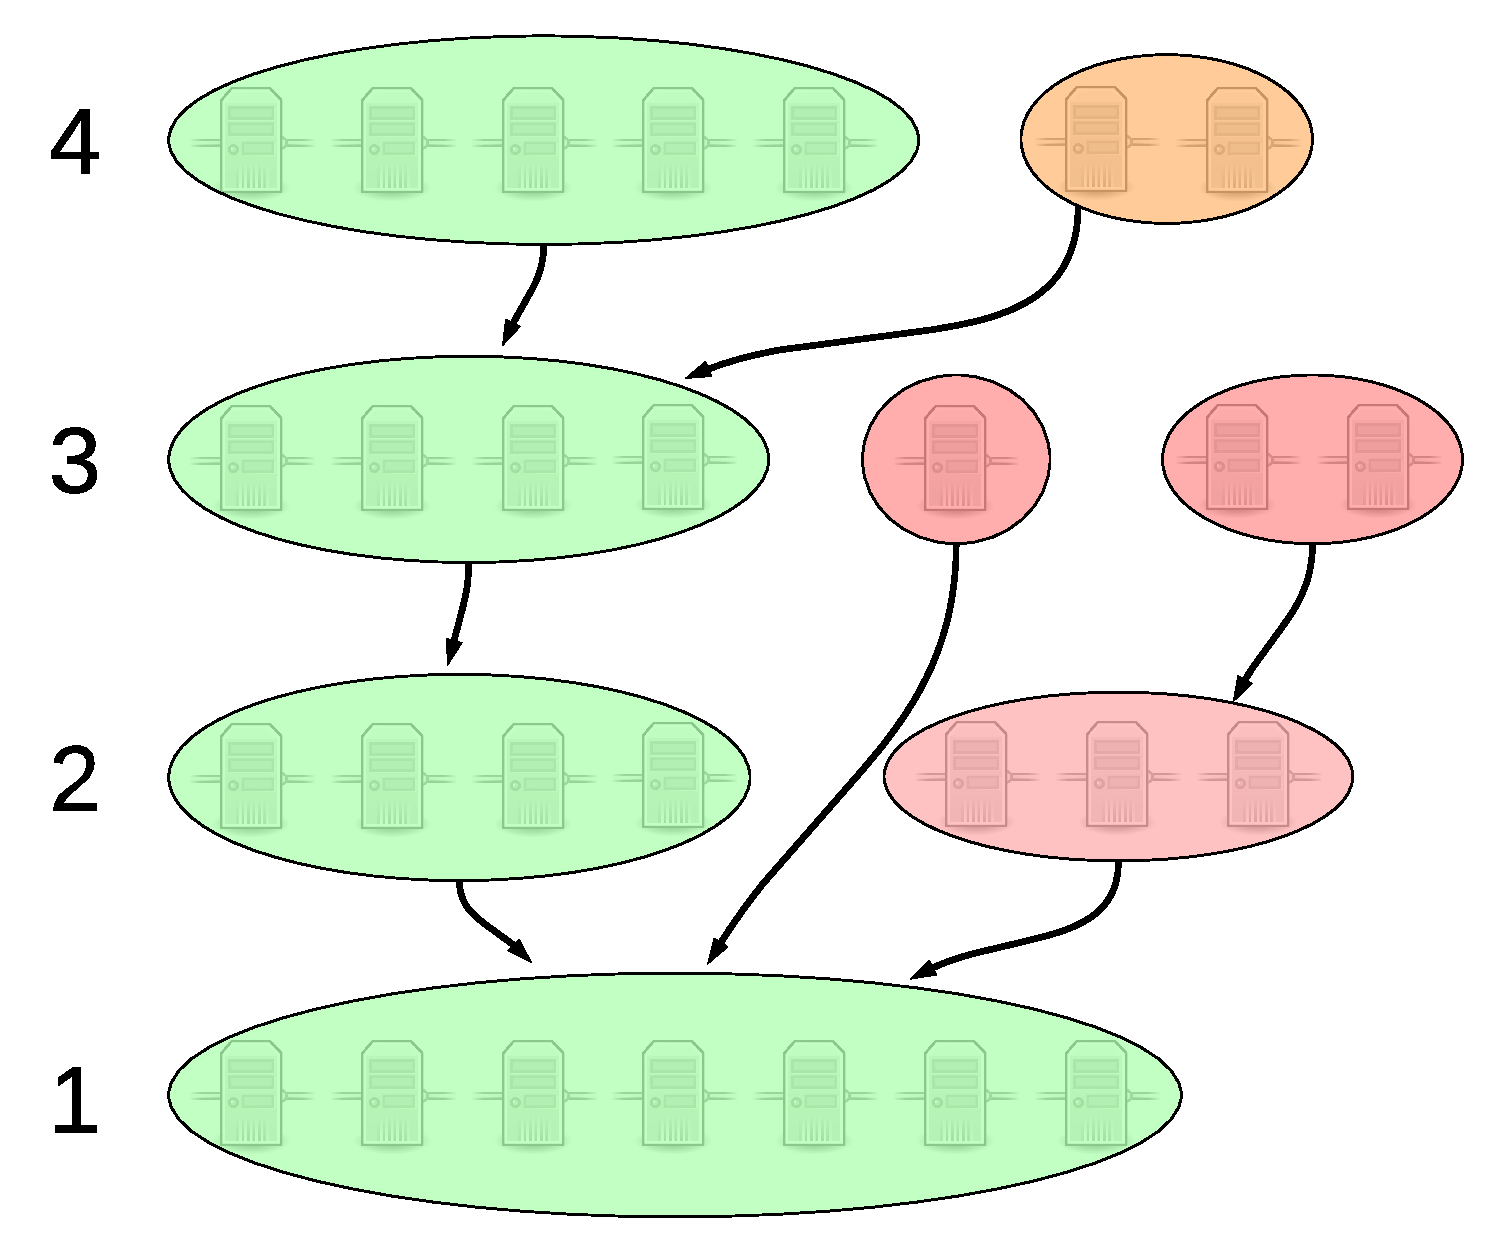
\includegraphics[width=0.7\linewidth]{../images/LucidCharts/Page-chain2.pdf}
	\caption{An example Pagechain across four Quorums with three side-chains. The valid master Pagechain from honest Quorum nodes (green) resists corruption from maliciously-colluding nodes (red) and malfunctioning nodes (orange).}
	\label{fig:sideChains}
\end{figure}

%\setlength{\belowcaptionskip}{-10pt}
\begin{figure}[h!]
	\centering
	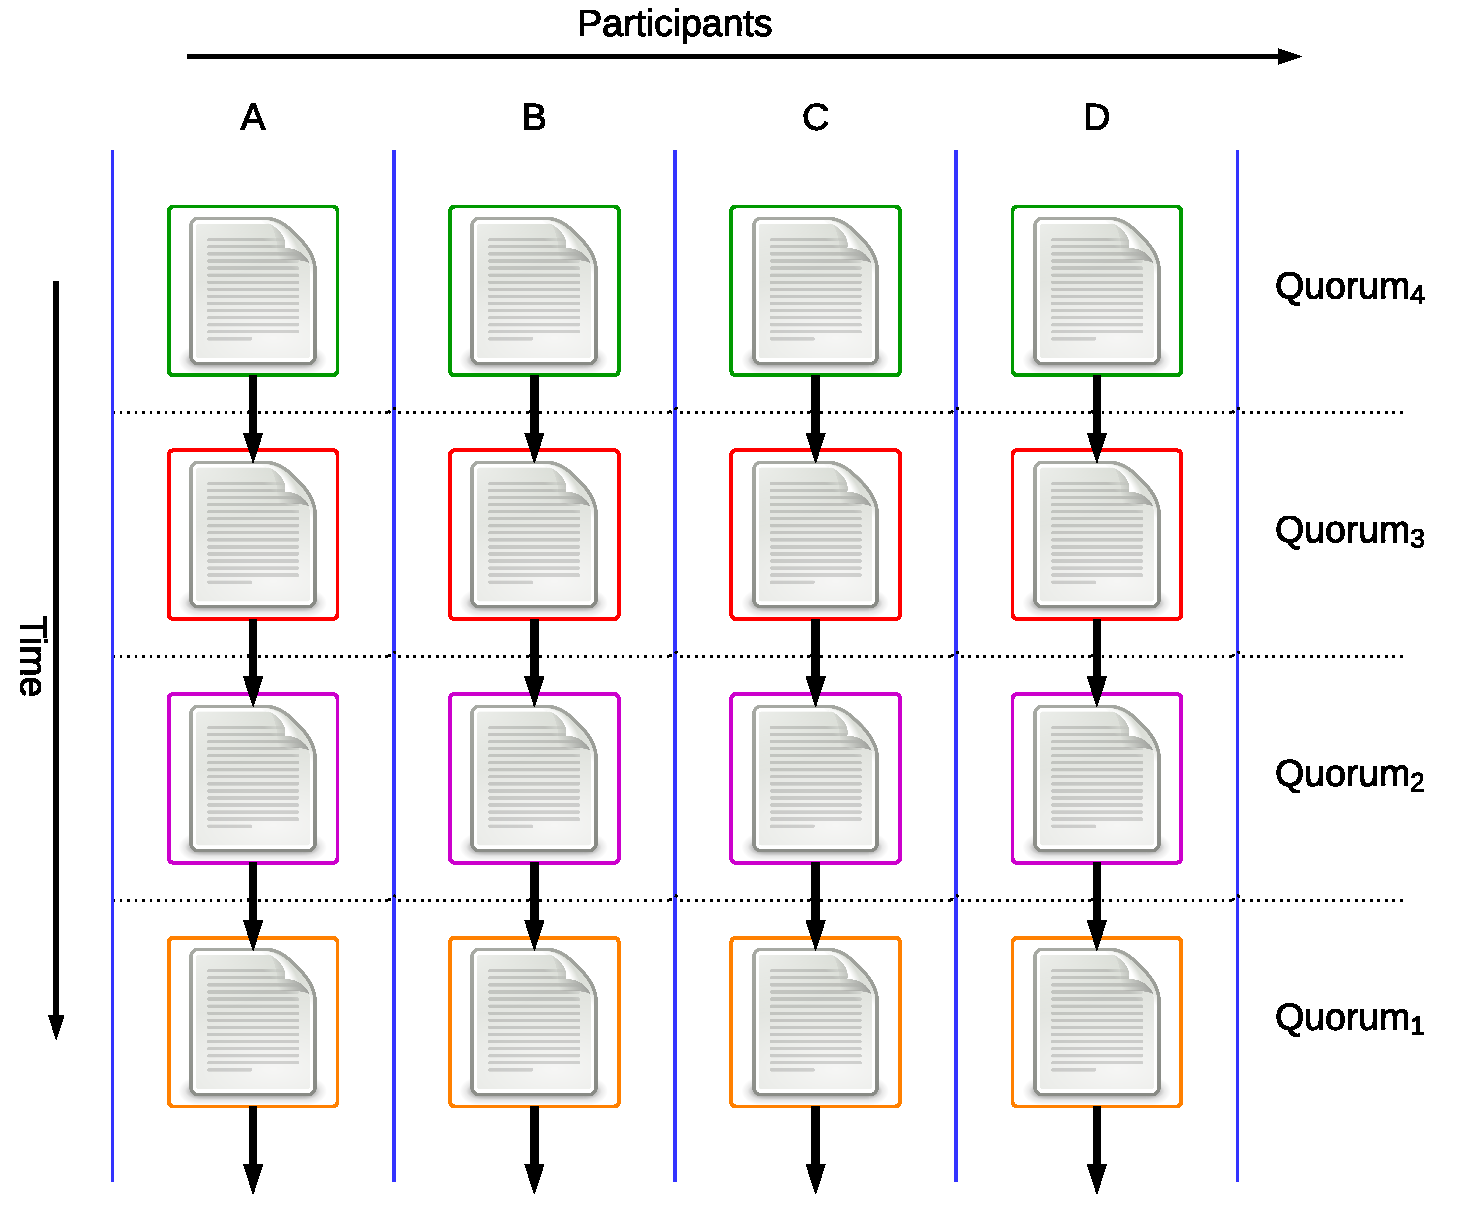
\includegraphics[width=0.9\linewidth]{../images/LucidCharts/Data-Structure-Overview.pdf}
	\caption{The master Pagechain is one-dimensional but spans across the network as each Mirror holds a copy. Each Page is maintained by a respective Quorum.}
\end{figure}

\begin{table}[h]
	\begin{tabular}{ | l | l | } \hline
    	$ L_{Q} $ & the size of the Quorum \\ \hline
    	$ L_{T} $ & the number of routers in the Tor network \\ \hline
    	$ L_{P} $ & the maximum number of Pages in the Pagechain \\ \hline
    	$ q $ & the Quorum iteration counter \\ \hline
    	$ \Delta q $ & the lifetime of a Quorum in days \\ \hline
    	$ s $ & the Snapshot iteration counter \\ \hline
    	$ \Delta s $ & the lifetime of a Snapshot in minutes \\ \hline
  	\end{tabular}
  	\caption[Table caption text]{Frequently used notations}
\end{table}

\subsection{Protocols}

We now describe the protocols fundamental to OnioNS functionality.

\subsubsection{Quorum Qualification}

Quorum Candidates must prove that they are both up-to-date Mirrors and that they sufficient capabilities to handle the increase in communication and processing from OnioNS protocols.

The na\"{i}ve solution to demonstrating the first requirement is to simply ask Mirrors for their Page, and then compare the recency of its latest Page against the Pages from the other Mirrors. However, this solution does not scale well; Tor has $ \approx $ 2.25 million daily users\cite{TorMetrics}: it is infeasible for any single node to handle queries from all of them. Instead, let each Mirror first calculate $ t = H(\mathit{pc} \concat \floor[\big]{\frac{m - 15}{30}}) $ where \emph{pc} is the Mirror's Pagechain and $ m $ is the number of minutes elapsed in that day, then include $ t $ in the Operator Contact field in his relay descriptor. Tor's consensus documents are published at the top of each hour; we manipulate $ m $ such that $ t $ is consistent at the top of each hour even with at most a 15-minute clock-skew. We suggest placing $ t $ inside a new field within the router descriptor in future work, but our use of the Contact field eases integration with existing Tor infrastructure. OnionNS would not be the first system to embed special information in the Operator Contact field: PGP keys and BTC addresses commonly appear in the field, especially for high-performance routers.

Tor's infrastructure already provides a mechanism for demonstrating the latter requirement; Quorum Candidates must also have the Fast, Stable, Running, and Valid flags. As of February 2015, out of the $ \approx $ 7,000 nodes participating in the Tor network, $ \approx $ 5,400 of these node have these flags and meet the latter requirement.\cite{TorMetrics}

\subsubsection{Quorum Formation}

Quorum Candidate Tor routers can determine in  $ \mathcal{O}(L_{T}) $ time if they have been chosen as part of the current Quorum. By the same procedure, clients can derive the Quorum in the past or present. Let Charlie be a Quorum Candidate.

\begin{enumerate}[noitemsep,nolistsep]
	\item Charlie obtains the consensus documents, $ cd $, published on day $ \floor[\big]{\frac{q}{\Delta q}} $ at 00:00 UTC.
	\item Charlie scans $ cd $ and constructs a list \emph{qc} of Quorum Candidates that have the Fast, Stable, Running, and Valid flags and that are in the largest set of Tor routers that publish an identical time-based hash.
	\item Alice constructs $ f = \mathit{R}(H(\mathit{cd})) $.
	\item Alice uses \emph{f} to randomly scramble \emph{qc}.
	\item The first $ \mathrm{min}(\mathrm{size}(\mathit{qc}), L_{Q}) $ routers are the Quorum.
\end{enumerate}

\subsubsection{Record Generation}

Bob must first generate a valid Record to claim a second-level domain name for his hidden service. The validity of his Record is checked by Quorum Nodes, Mirrors, and clients, so Bob must follow this protocol.

\begin{enumerate}[noitemsep,nolistsep]
	\item Bob constructs the \emph{nameList} domain-destination associations. He must include at least one second-level domain name. Each domain name can be up to 128 characters and contain any number of names.
	\item Bob optionally provides his PGP key fingerprint in \emph{contact}.
	\item Bob sets \emph{consensusHash} to the output of $ H(x) $, where $ x $ is the consensus documents published at 00:00 UTC on day $ \floor[\big]{\frac{q}{\Delta q}} $.
	\item Bob initially defines \emph{nonce} as four zeros.
	\item Let $ \mathit{central} $ be $\mathit{type} \concat \mathit{nameList} \concat \mathit{contact} \concat \mathit{timestamp} \concat \mathit{consensusHash} \concat \mathit{nonce} $.
	\item Bob sets \emph{pow} as $ \mathrm{PoW}(\mathit{central}) $.
	\item Bob sets \emph{recordSig} as the output of $ S_{\mathit{RSA}}(m, r) $ where $ m = \mathit{central} \concat \mathit{pow} $ and $ r $ is Bob's private RSA key.
	\item Bob saves the PKCS.1 DER encoding of his RSA public key in \emph{pubHSKey}.
\end{enumerate}

The Record is valid when $ H(\mathit{central} \concat \mathit{pow} \concat \mathit{recordSig}) \leq 2^{\mathit{d} * \mathit{c}} $ where \emph{d} is a fixed constant that specifies the work difficulty and \emph{c} is the number of second-level domain names claimed in the Record. This also requires Bob to increment \emph{nonce} and resign his Record at every iteration of $ \mathrm{PoW}(\mathit{central}) $.

\subsubsection{Record Processing}

A Quorum node $ Q_{j} $ listens for new Records from hidden service operators. When a Record $ r $ is received, $ Q_{j} $

\begin{enumerate}[noitemsep,nolistsep]
	\item $ Q_{j} $ rejects $ r $ if the Record is not valid.
	\item $ Q_{j} $ rejects $ r $ if any destination .onion addresses have no matching hidden service descriptor.
	\item $ Q_{j} $ rejects $ r $ if any of its second-level domains already exist in $ Q_{j} $'s Pagechain.
	\item $ Q_{j} $ informs Bob that $ r $ has been accepted.
	\item $ Q_{j} $ merges $ r $ into its current Snapshot.
	\item $ Q_{j} $ regenerates \emph{snapshotSig}.
\end{enumerate}

Then every $ \Delta s $ minutes each Quorum node floods its Snapshot to all other Quorum nodes, merges in Snapshots from other Quorum nodes into its Page, and generates a fresh Snapshot.

\subsubsection{Page Selection}

New Quorum nodes must select a Page from the previous Quorum to reference when generating a fresh Page. To reduce the chances of compromise, we select based on our last security assumption. Let Charlie be a Mirror.

\begin{enumerate}[noitemsep,nolistsep]
	\item Charlie obtains the set of Pages maintained by $ \mathit{Quorum}_{q} $.
	\item Charlie obtains the consensus $ \mathit{cd} $ issued on day $ \floor[\big]{\frac{q}{\Delta q}} $ at 00:00 UTC and authenticates it.
	\item Charlie uses $ \mathit{cd} $ to derive the Quorum.
	\item For each Page,
		\begin{enumerate}[noitemsep,nolistsep]
			\item Charlie asserts that $ \mathit{fingerprint} \in \mathit{Quorum}_{q} $.
			\item Charlie asserts that \emph{prevHash} references $ \mathrm{Page}_{q-1} $ found by this protocol.
			\item Charlie calculates $ h = H(\mathit{prevHash} \concat \mathit{recordList} \concat \mathit{consensusHash}) $.
			\item Charlie asserts that $ V_{\mathit{ed}}(h, E) $ returns true.
		\end{enumerate}
	\item Charlie sorts the set of Pages by the number of routers that have signed $ h $.
	\item For each Page in each $ h $,
		\begin{enumerate}[noitemsep,nolistsep]
			\item Charlie checks that $ \mathit{consensusHash} = H(\mathit{cd}) $.
			\item Charlie checks the validity of each Record in \emph{recordList}.
		\end{enumerate}
	\item If the validation of a Page fails, Charlie continues to the next $ h $.
	\item If the Page is valid, the next \emph{prevHash} references it.
\end{enumerate}

\subsubsection{Domain Query}

Alice needs only Bob's Record to contact Bob by his meaningful domain name. Let Alice type a domain $ d $ into the Tor Browser.

\begin{enumerate}[noitemsep,nolistsep]
	\item Alice constructs a Tor circuit to Charlie.
	\item \label{step:ask} Alice asks Charlie for the most recent Record $ r $ containing $ d $.
	\item Charlie finds and returns $ r $ to Alice and the components of the Merkle tree $ T $ described in section \ref{sec:authDenial}.
	\item If $ r $ is not found, Alice asserts that the second-level name of $ d $ is not found in $ T $, as otherwise Charlie is dishonest.
	\item If $ r $ is found, Alice asserts that $ r $ is valid and contained in $ T $, as otherwise Charlie is dishonest.
	\item If $ d $ in $ r $ points to a domain with a .tor pseudo-TLD, $ d $ becomes that destination and Alice jumps to step \ref{step:ask}.
	\item Alice asserts that the destination uses a .onion pseudo-TLD and contacts Bob by the traditional hidden service protocol.
	\item Alice extracts Bob's key from his hidden service descriptor and asserts that it matches $ r $'s \emph{pubHSKey}.
	\item Alice sends the original $ d $ to the hidden service.
\end{enumerate}

Alice may also request additional information from Charlie, providing her with more authenticity verification at the expense of additional networking and processing costs. Alice may ask for the Page $ p $ containing $ r $, which she can verify and authenticate against a single Quorum node, but she cannot check the last security assumption. Since $ p $'s \emph{pageSig} is a signature on $ h = H(\mathit{prevHash} \concat \mathit{recordList} \concat \mathit{consensusHash}) $, she may also ask for all $ h $s and all \emph{pageSig}s and assert that the Page Selection protocol derives $ p $. However, she does not have enough information to verify the integrity of $ p $'s \emph{prevHash}. Lastly, Alice may become certain that $ r $ is authentic and that $ d $ is unique by performing a synchronization against the OnioNS network and checking the Pagechain herself, but this is impractical in most environments. Tor's median circuit speed is often less than 4 Mbit/s,\cite{TorMetrics} so for the sake of convenience data transfer must be minimized. Therefore Alice can simply fetch minimal information and rely on her existing trust of members of the Tor network.

\subsubsection{Onion Query}

OnioNS also supports reverse-hostname lookups. In an Onion Query, Alice issues a hidden service address $ \mathit{addr} $ to Charlie and receives back all Records that have $ \mathit{addr} $ as a destination in their \emph{nameList}. Alice may obtain additional verification on the results by issuing Domain Queries on the source .tor domains. We do not anticipate Onion Queries to have significant practical value, but they complete the symmetry of lookups and allow OnioNS domain names to have Forward-Confirmed Reverse DNS matches. We suggest caching destination hidden service addresses in a digital tree (trie) to accelerate this lookup; a trie turns the lookup from $ \mathcal{O}(n) $ to $ \mathcal{O}(1) $, while requiring $ \mathcal{O}(n) $ time and $ \mathcal{O}(n) $ space to pre-compute the cache.

\subsection{Authenticated Denial-of-Existence}
\label{sec:authDenial}

In any system that serves authenticable names, a name server can prove a claim on the existence of a name by simply returning it. An often overlooked problem is ensuring that name servers cannot claim false negatives on resolutions; clients must be able to authenticate a denial-of-existence claim. Extensions to DNSSEC attempt to close this attack vector, but DNSSEC is not widely deployed, and we are not aware of any alternative DNS that addresses this. Although Alice may download the entire Pagechain and prove non-existence herself, we do not consider this approach practical in most realistic environments. Instead, we introduce a mechanism for authenticating denial-of-existence with minimal networking costs. To our knowledge this represents the first alternative DNS to authenticate denial-of-existence claims on domains en-masse.

We suggest reducing the networking costs with a Merkle tree\cite{merkle1988digital} $ T $. Let each Quorum node

\begin{enumerate}[noitemsep,nolistsep]
	\item Construct an array list \emph{arr}.
	\item For each second-level domain $ c $ in each Record $ r $ in the Pagechain, add $ c \concat H(r) $ to \emph{arr}.
	\item Sort \emph{arr}.
	\item Construct a Merkle tree $ T $ from \emph{arr}.
	\item Generate $ \mathit{sig}_{T} = S_{\mathit{ed}}(t \concat r, e) $ where $ t $ is a timestamp and $ r $ is the root hash of $ T $.
\end{enumerate}

As Records contain both second-level domains and their subdomains, $ T $ needs only contain $ c $ to reference all domains in $ r $, which further saves space. Then during a Domain Query Alice may use $ T $ to authenticate a domain $ d $ and verify non-existence for a Record $ r $.

\begin{enumerate}[noitemsep,nolistsep]
	\item Alice extracts the second-level name $ c $ from $ d $.
	\item If $ r $ exists, Charlie returns the leaf node containing $ r $ and all the tree nodes from leaf $ r $ to the root and their sibling nodes, so that Alice can verify authenticity of $ r $ by recomputing the root hash and verify that the largest subset of Quorum nodes signed the same root hash.
	\item If Charlie claims non-existence of $ c $, he returns two adjacent leaves $ a $ and $ a $ (and the nodes on their paths and siblings) such that $ a < c < b $, or in the boundary cases that $ a $ is undefined and $ b $ is the left-most leaf or $ b $ is undefined and $ a $ is the right-most leaf.
	\item If either assertion fails, Charlie is dishonest.
\end{enumerate}

The Quorum must regenerate $ T $ every $ \Delta T $ hours to include new Records. Then Alice needs only fetch the signatures on $ T $ at least every $ \Delta T $ hours to ensure that she can authenticate new Records during the Domain Query. Thus $ \Delta T $ is the primary factor in the speed of Record propagation: Alice cannot authenticate or verify denial-of-existence claims on Records newer than $ \Delta T $. Alice must also fetch the $ L_{Q} $ signature from all Quorum nodes and assert that $ T $ is signed by the largest set of nodes maintaining the same Page, in correspondence with our last security assumption.

We note that a sorted Merkle tree does not support efficient dynamic record updates. The tree needs to be rebuilt to handle updates. To support efficient record update in $ \mathcal{O}(\mathrm{log}(n)) $ time, we can adopt the skip list data structure proposed in \cite{goodrich2001implementation}. Proof of existence and non-existence still works in a similar way.

\section{Security Analysis}
\label{sec:Analysis}

In this section, we analyse the security of the OnioNS system with regard to our security goals. First, the registrations and client queries are anonymous because they occur over a Tor circuit, which we assume provides privacy and anonymity. No identifiable information is leaked from the data contents as well. Second, registrations are authenticable, which can be reduced to the security of the Merkle hash tree and to the assumption that the largest subset of Quorum nodes are honest. We verify this assumption in section \ref{sec:QSelection} and \ref{sec:QSize}. Domain uniqueness also stems from the above assumption, relying on honesty of Quorum nodes to avoid collisions. Quorum selection is a random process assuming sufficient entropy in the Tor consensus, which we verify in section \ref{sec:entropy}. We also highlight the potential for the leakage of the .tor pseudo-TLD on the Internet DNS.

\subsection{Quorum Selection}
\label{sec:QSelection}

% check math, symbols for number of Quorum Candidates

In section \ref{sec:threatModel}, we assume that an attacker, Eve, controls some fixed $ f_{E} $ fraction of routers on the Tor network. Quorum selection may be considered as an $ L_{Q} $-sized random sample taken from an $ L_{T} $-sized population without replacement, where the population contains a subset of $ L_{Q} * f_{E} $ entities that we assume are compromised and colluding. If our selection includes $ L_{E} $ Eve-controlled routers, then Eve controls the Quorum if either $ > \frac{L_{Q} - L_{E}}{2} $ honest Quorum nodes disagree or if $ L_{E} > \frac{L_{Q}}{2} $. The former scenario is hard to model theoretically or in simulation, but the probability of the latter can be statistically calculated. The Quorum is short-lived and changed every $ \Delta q $ days, so we must consider the implications of selections for both $ L_{Q} $ and $ \Delta q $.

\subsubsection{Quorum Size}
\label{sec:QSize}

The probability that Eve controls $ L_{E} $ Quorum nodes is given by the hypergeometric distribution, whose probability mass function (PMF) is shown in Equation \ref{eq:hypergeoPMF}.

Then the probability that $ L_{E} > \frac{L_{Q}}{2} $, a complete compromise of the Quorum, is given by Equation \ref{eq:compromiseProb}. Odd choices for $ L_{Q} $ prevents the network from splintering in the event that the Quorum is evenly split across two Pages. We assume that $ L_{Q} $ will be selected from a pool of 5,400 Quorum Candidates --- the number, as of May 2015, of Tor routers with the Fast and Stable flags. We provide the statistical calculations in Figure \ref{fig:quorumMajority}.

\begin{align}
	\mathrm{Pr}(L_{E}) &= \frac{\binom{f_{E}}{k}\binom{N - f_{E}}{L_{Q} - k}}{\binom{N}{L_{Q}}}
	\label{eq:hypergeoPMF}
	\\
	\mathrm{Pr}(L_{E} > \frac{L_{Q}}{2}) &= \displaystyle\sum_{x=\ceil{\frac{L_{Q}}{2}}}^{L_{Q}} \frac{\binom{f_{E}}{k}\binom{N - f_{E}}{L_{Q} - k}}{\binom{N}{L_{Q}}}
	\label{eq:compromiseProb}
\end{align}

% todo: 512 isn't in legend
\begin{figure*}
	\centering
	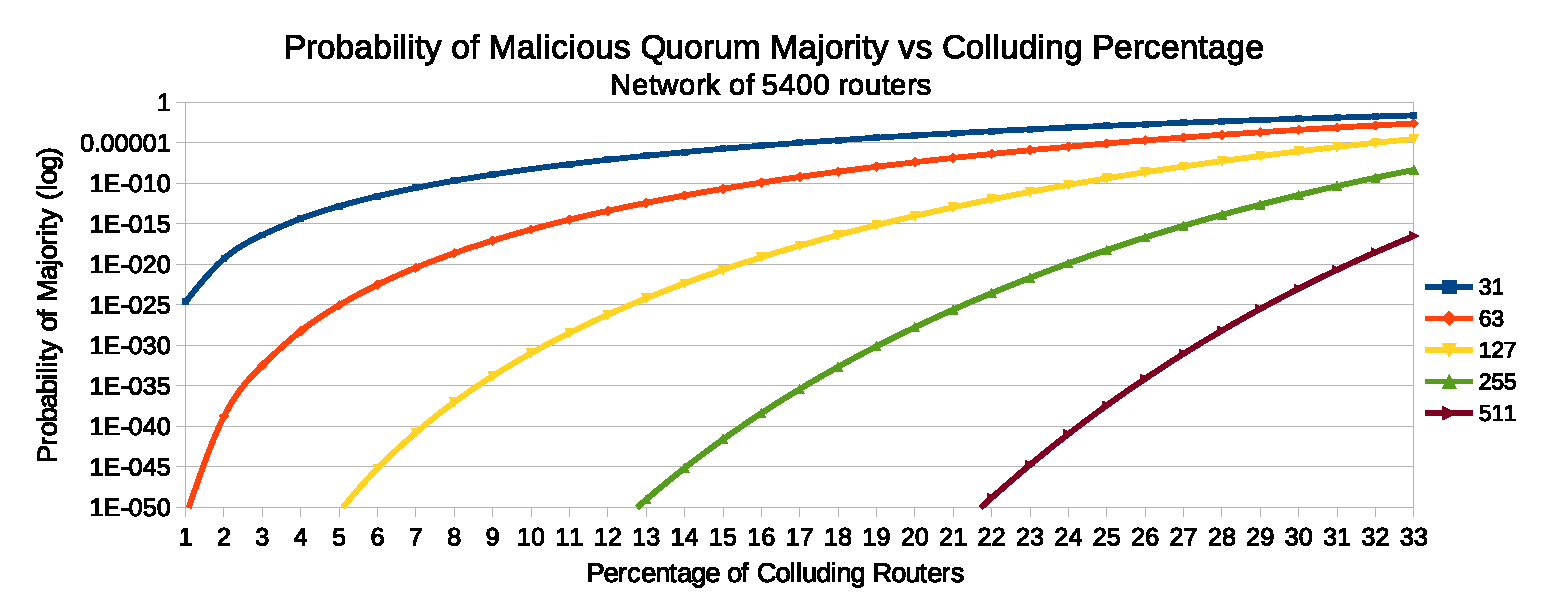
\includegraphics[width=0.75\linewidth]{../analysis/MaliciousQuorumProbability_tight.eps}
	\caption{We calculate the PMF of the hypergeometric distribution for a population of 5,400, $ f_{E} \in [1,33] $, and five selections for $ L_{Q} $: 31, 63, 127, 255, and 511. $ f_{E} > 33 $ represents a complete compromise of the Tor network, so we do not consider values beyond this range.}
	\label{fig:quorumMajority}
\end{figure*}

Figure \ref{fig:quorumMajority} shows that choices of $ L_{Q} = 31 $ and $ L_{Q} = 63 $ are suboptimal, they quickly grow for even low levels of $ f_{E} $. Small Quorums are also more susceptible to DDoS attacks. We feel it safe to discard threats that have probabilities $ \leq \frac{1}{2^{128}} \approx 10^{-38.532} $ --- the probability of Eve randomly guessing a 128-bit AES key. $ L_{Q} = 31 $ exceeds this with more than one percent collusion, $ L_{Q} = 63 $ above two percent, and $ L_{Q} = 127 $, $ L_{Q} = 255 $, and $ L_{Q} = 511 $ at $ \geq 7.7 $, $ \geq 16.1 $, and $ \geq 24.6 $ percent, respectively. Therefore we recommend setting $ L_{Q} \geq 127 $.

\subsubsection{Quorum Rotation}

In section \ref{sec:threatModel}, we assume that $ f_{E} $ is fixed and does not increase in response to the inclusion of OnioNS on the Tor network. If we also assume that $ L_{T} $ is fixed, then we can examine the impact of choices for $ \Delta q $ and calculate the probability of Eve compromising \emph{any} Quorum over a long period of time $ t $. Smaller values for $ \Delta q $ implies that we select more Quorums over that time period and thus increase our cumulative chances of compromise, but it also reduces the disruption timeline for a malicious Quorum. Eve's cumulative chances of compromising any Quorum is given by $ 1 - (1 - \frac{f_{E}}{L_{T}})^t $. We estimate this over 10 years in Figure \ref{fig:cumulativeProbability}.

\begin{figure}[h]
	\centering
	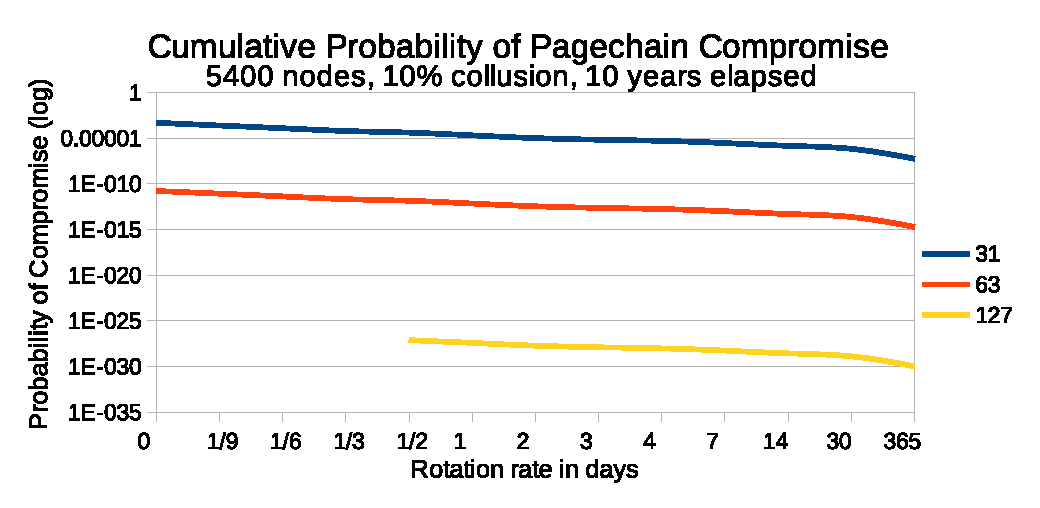
\includegraphics[width=\linewidth]{../analysis/CumulativeMaliciousQuorum_tight.eps}
	\caption{The cumulative probability that Eve controls any Quorum at different rotation rates over 10 years at $ f_{E} = 10 $. We do not consider $ L_{Q} = 255 $ or $ L_{Q} = 511 $ as they produce values less than $ 10^{-58} $ and $ 10^{-134} $, respectively, far below our $ 10^{-38.532} $ threshold.}
	\label{fig:cumulativeProbability}
\end{figure}

Figure \ref{fig:cumulativeProbability} suggests that although lower values of $ \Delta q $ negatively impact security, the choice of $ L_{Q} $ is more significant. It also supports our earlier conclusion that the choices of $ L_{Q} = 31 $ and $ L_{Q} = 63 $ are suboptimal. Based on Figure \ref{fig:cumulativeProbability} we further reiterate our recommendation of $ L_{Q} \geq 127 $ and suggest $ \Delta q \geq 1 $. Although a malicious Quorum would have the capabilities to deploy a variety of attacks on the network, the proper selections of $ L_{Q} $ and $ \Delta q $ reduces the likelihood of this occurring to near-zero probabilities. We consider this a stronger solution than introducing countermeasures to specific Quorum-level attacks.

\subsubsection{Entropy Estimation}
\label{sec:entropy}

% todo: \emph vs \textit

Periodically, Tor routers upload signed \emph{descriptors} --- routing information, cryptographic keys, and other information --- to Tor's directory authorities (dirauths). Once per hour, the dirauths aggregate and republish the descriptors back to the network, enabling Tor's network to be dynamic and distributing new information to all parties in an efficient and timely manner. We use Tor's network consensus as a global source of entropy, enabling the entire network to agree on a common Quorum. While Tor provides no guarantee that the network is using the same consensus at the same time, the consensus is timestamped, so we can reference it by their time of publication. We focus on two essential documents that clients assemble from the consensus: \emph{cached-certs} and \emph{cached-microdesc-consensus}. Although these documents contain other elements, for the sake of brevity we briefly describe their essential components.

\begin{itemize}[noitemsep,nolistsep]
	\item \textbf{cached-certs} A list of long-term identity and short-term signing RSA keys from each dirauth.
	\item \textbf{cached-microdesc-consensus} Essential information about each router, such as networking information and capabilities.
\end{itemize}

If \emph{cd} is $ \mathit{cached \mbox{--} certs} \concat \mathit{cached \mbox{--} microdesc \mbox{--} consensus} $, we initialize $ \mathit{R}(s) $ with the output of the $ H(\mathit{cd}) $. Eve may desire to find a hash $ k $ that generates a desirable Quorum, either one that includes her routers or excludes particular honest routers. As $ H(x) $ is SHA-384, SHA-384's strong resistance to preimage attack forces Eve to spend $ L_{T} * 2^{383} $ operations on average to find $ k $. Eve may also try to manipulate her router's descriptors such that $ H(\mathit{cd}_{q+1}) = k $, but SHA-384's resistance to second-preimage attacks also requires this to require $ L_{T} * 2^{383} $ operations as well. However, if \emph{cd} contains sufficient entropy, Eve is unable to predict the next Quorum or influence it to her favor. Since the dirauths publish a new consensus every hour, we must analyse the entropy rate between consecutive hours.

We constructed a first-order Markov model and estimated the entropy of the \emph{cached-microdesc-consensus} document by analysing the transitions for various fields between consecutive consensuses. We also provide analysis on the dynamics of the Tor network by counting routers that enter or leave the Tor network between consecutive consensuses in Figure \ref{fig:xorRouters}. Here we identity routers by their identity keys; just as Tor does, we consider routers that change their identity keys as two different routers; one leaving and one entering the network. Routers entering the network introduce significant amounts of information into the consensus. For example, \emph{cached-microdesc-consensus} contains the 160-bit SHA-1 hash of the router's RSA-1024 identity key, which are generated through OpenSSL. Thus new routers contribute at least 160 bits of information. Figure \ref{fig:xorRouters} suggests that we may expect approximately 100 to 175 routers to leave or enter the network per hour. Thus we may expect approximately 16,000 to 28,000 bits of entropy per hour from this dynamic.

\begin{figure}[h]
	\centering
	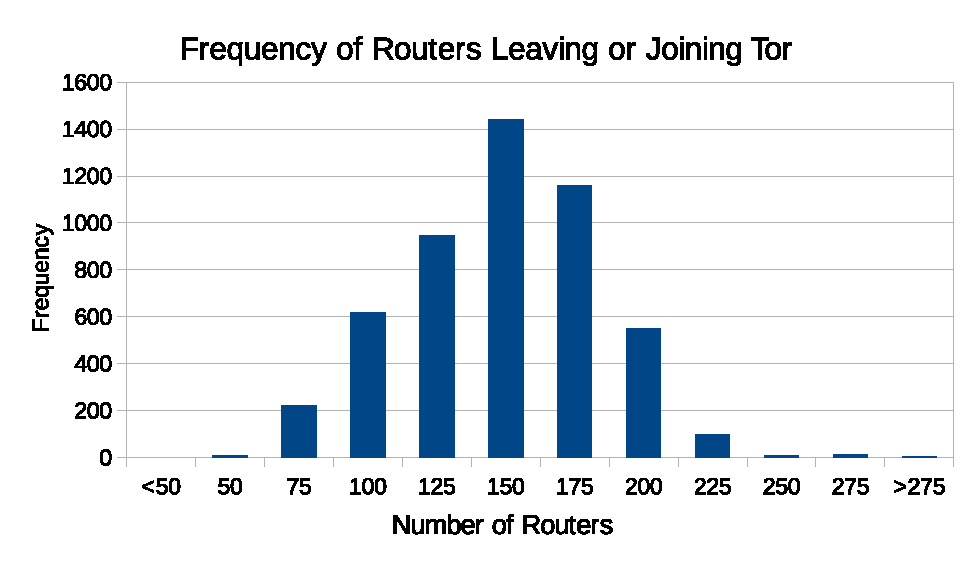
\includegraphics[width=\linewidth]{../analysis/LeaveJoinFrequency.eps}
	\caption{A histogram of the number of routers entering or leaving the network between consecutive consensuses across the seven-month period.}
	\label{fig:xorRouters}
\end{figure}

For routers that are present between consecutive pairs, we focus on six critical fields from each router's descriptor inside \emph{cached-microdesc-consensus}: \emph{nickname}, the router's name chosen by its operator or a default name; \emph{publication}, the time when it last published a descriptor; \emph{IP address}, its network address; \emph{ORPort}, the network port for onion routing; \emph{version}, the version of the Tor protocol that this relay is running; and \emph{bandwidth}, as self-reported or as measured by the dirauths. Tor routers change \emph{publication} when either 18 hours has elapsed since the last descriptor publication, its fields have changed, or if its uptime has been reset.

We obtained from \url{collector.torproject.org} 5,067 archived hourly publications of \emph{cached-microdesc-consensus} across a seven-month period between September 1, 2014 00:00 UTC and March 31, 2015 23:00 UTC. We construct a Markov model for the six aforementioned fields and illustrate the number of observed transitions for each field in Figure \ref{fig:transitionCount}.

\begin{figure}[h]
	\centering
	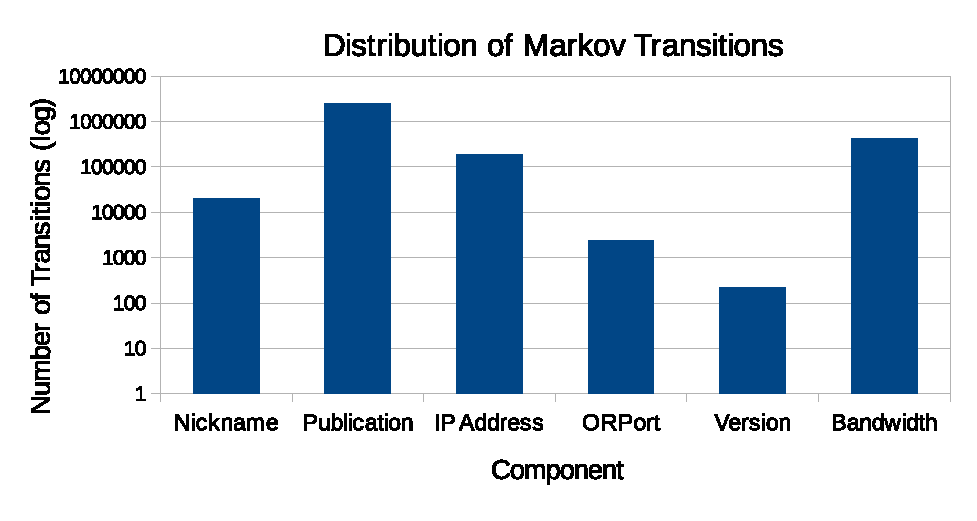
\includegraphics[width=\linewidth]{../analysis/MarkovTransitionDistribution.eps}
	\caption{The number of observed transitions for \emph{nickname}, \emph{publication}, \emph{IP address}, \emph{ORPort}, \emph{version}, and \emph{bandwidth} between consecutive consensuses across the seven-month period.}
	\label{fig:transitionCount}
\end{figure}

Then the entropy rate is given by equation \ref{eq:entropyRate}, where $ P_{i} $ is the probability of state $ i $ and $ P_{i}(j) $ is the probability of state $ j $ given $ i $ (the $ i $-$ j $ transition). We multiply the entropy rate by the total number of routers in the Tor network. This assumes that router's are independently and uniformly distributed, but this is not always the case as small sets of routers may be managed together and change as one. However, identifying these sets and analysing them separately is non-trivial to impossible; administrators may operate anonymously or try to purposely hide their management of multiple geographically-distance routers. Due to this, this assumption results in an estimation of the entropy and not an exact value. We calculate this rate estimation for each of the six fields and illustrate the results in Figure \ref{fig:entropyRates}.

\begin{equation}
\mathrm{H}(\mathcal{S}) = - L_{T} \sum_{i} P_{i} \sum_{j} P_{i}(j) \log_{2}P_{i}(j)
\label{eq:entropyRate}
\end{equation}

\begin{figure}[h]
	\centering
	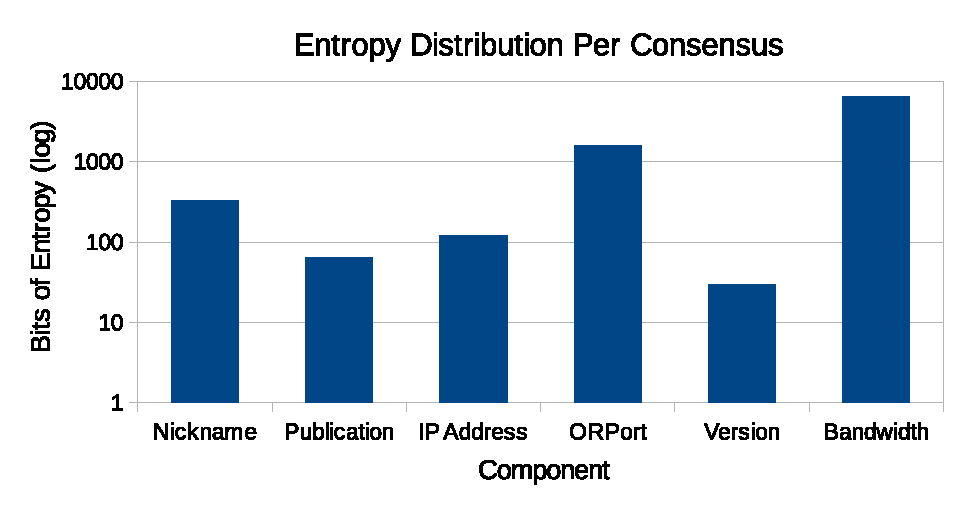
\includegraphics[width=\linewidth]{../analysis/EntropyDistribution.eps}
	\caption{The entropy rate distribution for each of the six fields in \emph{cached-microdesc-consensus}, scaled by the average size of the Tor network.}
	\label{fig:entropyRates}
\end{figure}

The average size of the Tor network across the seven-month period was 6,672 routers, thus together these fields contributed on average approximately 8,896.7 bits of entropy per hour across our seven-month view. The two documents contain at least this much entropy; our analysis does not comprehensively cover all the fields in \emph{cached-certs} and \emph{cached-microdesc-consensus}, so other fields may also contribute additional information. Based on this analysis, the approximately 16,000 to 28,000 entropy bits contributed hourly by routers joining or entering the Tor network, and our previous statistical calculations, we conclude that with $ L_{Q} \geq 127 $, the Quorum Formation protocol is secure under our design assumptions. Our analysis shows that the size and dynamic nature of the Tor network provides the strongest defence against Quorum-level attacks.

\subsection{Outsourcing Record Generation}

In the Record Generation protocol, we intentionally included the scrypt calculation inside the signing step in order to require Bob to run scrypt himself. However, our protocol does not entirely prevent Bob from outsourcing this expensive computation to a secondary resource, Craig, in all cases. We assume that Craig does not have Bob's private key. Then,

\begin{enumerate}[noitemsep,nolistsep]
	\item Bob creates an initial Record $ R $ and completes the \emph{type}, \emph{nameList}, \emph{contact}, \emph{timestamp}, and \emph{consensusHash} fields.
	\item Bob sends $ R $ to Craig.
	\item Let $ \mathit{central} $ be $\mathit{type} \concat \mathit{nameList} \concat \mathit{contact} \concat \mathit{timestamp} \concat \mathit{consensusHash} \concat \mathit{nonce} $.
	\item Craig generates a random integer $ K $ and then for each iteration $ j $ from 0 to $ K $,
		\begin{enumerate}[noitemsep,nolistsep]
			\item Craig increments \emph{nonce}.
			\item Craig sets \emph{PoW} as $ \mathrm{PoW}(\mathit{central}) $.
			\item Craig saves the new $ R $ as $ C_{j} $.
		\end{enumerate}
	\item Craig sends all $ C_{0 \le j \le K} $ to Bob.
	\item For each Record $ C_{0 \le j \le K} $ Bob computes
		\begin{enumerate}[noitemsep,nolistsep]
			\item Bob sets \emph{pubHSKey} to his public RSA key.
			\item Bob sets \emph{recordSig} to $ S_{\mathit{RSA}}(m, r) $ where $ m = \mathit{central} \concat \mathit{pow} $ and $ r $ is Bob's private RSA key.
			\item Bob has found a valid Record if $ H(\mathit{central} \concat \mathit{pow} \concat \mathit{recordSig}) \leq 2^{\mathit{d} * \mathit{c}} $
		\end{enumerate}
\end{enumerate}

% todo: calculate chances of Craig computing a correct record

However, this ensures that ensures that Craig must always compute more scrypt iterations than necessary; Craig cannot generate \emph{recordSig} and thus cannot compute if the hash is below the threshold. Moreover, the scrypt work incurs a cost onto Craig that must be compensated financially by Bob. Thus the Record Generation protocol always places a cost on Bob.

\subsection{DNS Leakage}

Accidental leakage of .tor lookups over the Internet DNS via human mistakes or misconfigured software may compromise user privacy. This vulnerability is not limited to OnioNS and applies to pseudo-TLD; Mohaisen and Thomas observed .onion lookups on root DNS servers at a frequency that corresponded to external global events and highlighting the human factor in those leakages.\cite{thomasmeasuring} Closing this leakage is difficult; arguably the simplest approach is to introduce whitelists or blacklists into common web browsers to prevent known pseudo-TLDs from being queried over the Internet DNS. Such changes are outside the scope of this work, but we highlight the potential for this attack.

\section{Evaluation}
\label{sec:eval}

\subsection{Implementation}

We have built a partial reference implementation of OnioNS in C++11, primarily the Record Generation and Domain Query protocols. Botan provides the implementation of our cryptographic operations, Boost Asio provides our networking engine, and Linux libjsoncpp-dev library provides implementations of JSON encoding and decoding. We encode all the data structures in JSON; JSON is significantly more compact than XML, but retains user readability and its support of basic primitive types is highly applicable to our needs. Our code is available under the Modified BSD License. % at \url{https://github.com/Jesse-V/OnioNS}.

% todo: need to test verifying agreement from multiple Quorum nodes

We implemented the essential functionality for Bob, Charlie, and Alice. We used the Shallot\cite{KatmagicShallot} vanity key generator to find an RSA key that hashed to a hidden service address with the ``OnioNS'' prefix. Shallot found ``onions55e7yam-27n.onion''. We constructed a website and attached Tor to the nginx web server. Then we loaded the private key into OnioNS and constructed a Record containing an association between ``example.tor'' and ``onions55e7yam27n.onion''. Next, we transmit this Record to a fixed server over a Tor circuit and started a TCP server to respond to Domain Queries. Finally, we modified Tor such that when Alice types ``example.tor'' into the Tor Browser, Tor intercepts the pseudo-TLD and sends it via IPC to the OnioNS client. Then the OnioNS client performs a Domain Query to Charlie and writes ``onions55e7yam27n.onion'' back to the Tor client over IPC. Finally, Tor rewrites the original ``example.tor'' lookup to ``onions55e7yam27n.onion'' and contacts our hidden service over the traditional Tor protocol. Tor performs asynchronously here; it must place the lookup on hold, free its event loop to avoid a deadlock, and asynchronously resume the lookup once it receives the response. From the user's perspective, the content of \url{http://onions55e7yam27n.onion} loads transparently under the \url{http://example.tor} URL.

%\begin{figure}[h]
%	\centering
%	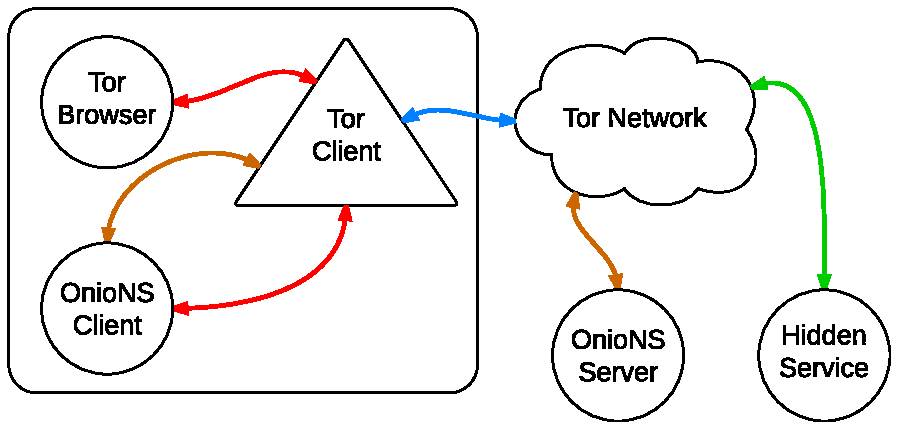
\includegraphics[width=0.6\linewidth]{../images/LucidCharts/OnioNS_Prototype.pdf}
%	\caption{The unresolved .tor pseudo-TLD travels (red) from the Tor Browser to the OnioNS client. The client issues a Domain Query (orange) to a remote server, who returns a Record. The client returns the .onion address to Tor, which then contacts the HS (green).}
%	\label{fig:prototypeDiagram}
%\end{figure}

\begin{figure}[h]
	\centering
	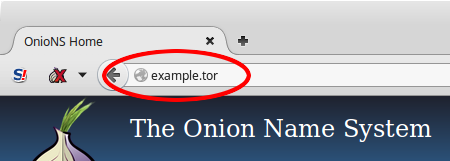
\includegraphics[width=0.9\linewidth]{../images/example.png}
	\caption{We load the OnioNS' hidden service, onions55e7yam27n.onion, transparently under the ``example.tor'' domain on Tor Browser 4.5.1, a fork of Firefox ESR 31.7.0.}
	\label{fig:prototypeExample}
\end{figure}

We conducted several performance measurements for the Record Generation and Domain Query protocols. Our experiment involves two machines, A and B. Both were hosted on 1 Gbit connections on a university campus. Machine A has an Intel Core2 Quad Q9000 (Penryn architecture) @ 2.00 GHz CPU from late 2008 and Machine B has an Intel i7-2600K (Sandy Bridge architecture) @ 4.3 GHz CPU from 2011, representing low-end and medium-end consumer-grade computers, respectively. We hosted our hidden service and TCP server on Machine B.

\subsection{Results}

\subsubsection{Performance}

We selected the parameters of scrypt such that it consumed 128 MB of RAM during operation. We consider this an affordable amount of RAM for low-end consumer-grade computers. We created a multi-threaded implementation of the Record Generation protocol and used all eight virtual CPU cores on Machine B to generate our Record. As expected, our RAM consumption scaled linearly with the number of scrypt instances executed in parallel; we observed approximately 1 GB of RAM consumption during Record Generation. Then we measured the average CPU wall-time required for both machines to validate the Record.

\renewcommand{\arraystretch}{1}
\begin{center}
    \begin{tabular}{ | c | c | c | c |}
    \hline
    \textbf{Description} & \textbf{A (ms)} & \textbf{B (ms)} & \textbf{Samples} \\ \hline
    Parsing JSON & 5.21 & 2.42 & 100 \\ \hline
	Validating scrypt & 448.184 & 294.963 & 25 \\ \hline
	$ V_{\mathit{RSA}}(m, E) $ & 6.35 & 2.74 & 200 \\ \hline
	Total Time & 459.744 & 300.123 & 25 \\ \hline
    \end{tabular}
\end{center}

As expected, Machine B outperformed Machine A in all instances and we observed that single iteration of scrypt dominated the total validation time. This is a CPU cost introduced to Tor clients, Mirrors, and Quorum nodes for each Record.

Mirrors must also check the Page signatures from all $ L_{Q} $ Quorum nodes. We use Ed25519 to reduce the signature space requirements and CPU time required for verification: $ S_{\mathit{ed}}(m, e) $ signatures fit into 64 bytes and may be verified in batch form. Bernstein et al. reports that a quad-core Westmere-era CPU can generate 109,000 signatures per second and verify 71,000 signatures per second with 134,000 CPU cycles per signature.\cite{bernstein2011high}. Therefore, even with large Quorums, we anticipate Mirrors being able to verify Page signatures from all Quorums in sub-second time on moderate hardware.

\subsubsection{Latency}

We measure the latency introduced by the Domain Query protocol and compare against loading a hidden service via its traditional .onion addresses. Our experiment measured the time between when Tor received ``example.tor'' from the Tor Browser and when it first began loading our hidden service. We conducted 25 measurements. We restarted Tor between tests in order to utilize different circuits and also restarted the Tor Browser to flush browser-side caching.

\renewcommand{\arraystretch}{1}
\begin{center}
    \begin{tabular}{ | c | c | c | c |}
    \hline
    \textbf{Lookup} & \textbf{Fastest (s)} & \textbf{Slowest (s)} & \textbf{Mean (s)} \\
    \hline
    .onion & 6.1 & 8.5 & 7.1 \\ \hline
	.tor & 8.5 & 11.4 & 9.7 \\
	\hline
    \end{tabular}
\end{center}

Tor's latency is primarily dominated by circuit construction and negotiation with the hidden service. This time is highly dependent on the circuit's network distance and the speed of each Tor router. Our measurements include the time to build circuits to our TCP server and the Domain Query protocol, which includes a single call to scrypt and $ V_{\mathit{RSA}}(m, E) $. We avoid additional latency costs by implementing a DNS cache in order to allow subsequent queries to be resolved locally. In future work we will reduce the latency by recycling existing circuits that Tor constructs on startup and by moving the server to the circuit's exit router, eliminating an unnecessary network hop.

\section{Conclusions and Future Work}

We have presented the Onion Name System (OnioNS), a distributed, secure, and usable alternative DNS that maps globally-unique and meaningful .tor domains to .onion hidden service addresses, and achieve all three properties of Zooko's Triangle. We enable any hidden service operator to anonymously claim a human-readable name for their server and clients to query the system in privacy-enhanced manner. We introduce a distributed self-healing blockchain-based database and mechanisms that let clients authenticate and verify denial-of-existence claims. Additionally, we utilize the existing and semi-trusted infrastructure of Tor, which significantly narrows our threat model to already well-understood attack surfaces and allows our system to be integrated into Tor with minimal effort. Our reference implementation demonstrates high usability and shows that OnioNS successfully addresses the major usability issue that has been with Tor hidden services since their introduction in 2002.

In future work we will expand our implementation and pursuit integrating it into Tor. OnioNS requires a few changes to Tor, namely a new .tor pseudo-TLD and Ed25519 router keys, but we introduce no changes to Tor's hidden service protocol. Should Tor's developers introduce changes to the hidden service protocol, OnioNS can become forwards-compatible with a few changes. Additionally, our implementation currently only supports ASCII characters in domain names, so in future work we will explore implementing Punycode to provide support for international character sets. Unlike the Internet DNS, we will disallow digits zero and one (similar to base32 encoding) in order to reduce the threat of phishing attacks from spoofed domains with indistinguishable characters.

%\section{Acknowledgements}
%
%We would like to thank Tor developers Roger Dingledine, Yawning Angel, and Nick Mathewson for their assistance with Tor technical support.

%, a password-based key derivation function which is notable for its large memory and CPU requirements during its operation. The scrypt function provides significantly greater resistance to custom hardware attacks and massively parallel computation primarily due to its memory requirements. This limits attackers to the same software implementation and asymptotic cost as legitimate users.\cite{percival2009stronger}\cite{percival2012scrypt} We choose scrypt because of these advantages over other key derivation functions such as SHA-256 or PBKDF2. For these reasons scrypt is also common for proof-of-work purposes in some cryptocurrencies such as Litecoin.

\bibliographystyle{abbrv}
\bibliography{citations}

\end{document}
